

%  emu channel
\begin{figure}[ht]
    \centering
    $ \mu  e - 1b$ \\
    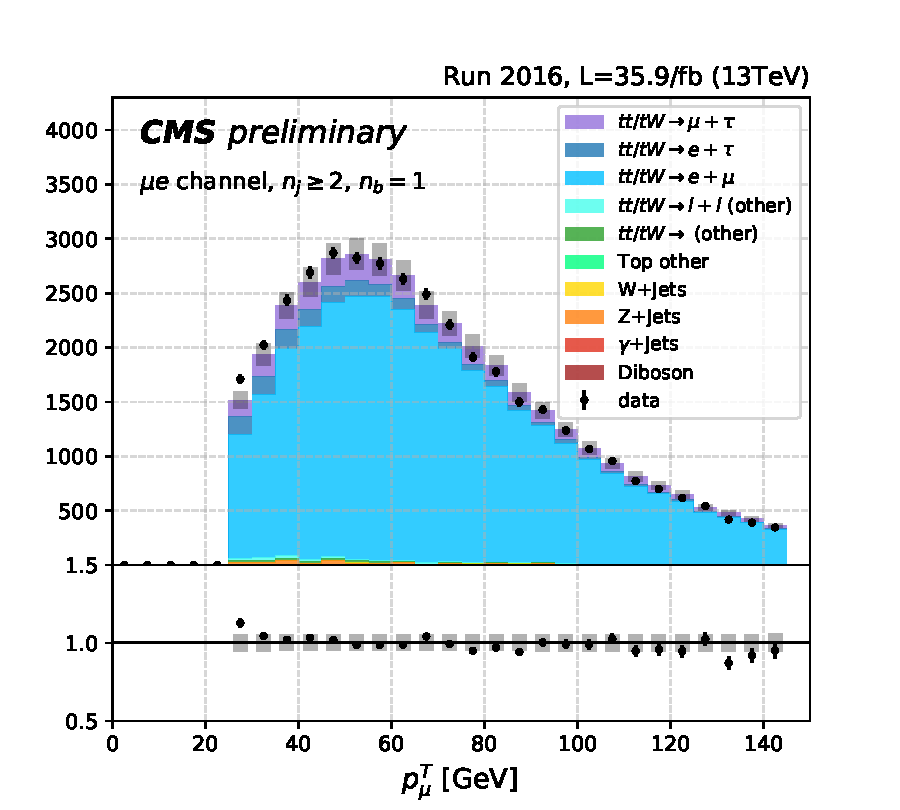
\includegraphics[width=0.49\textwidth]{chapters/Analysis/sectionPlots/figures/kinematics_pickles/emu/1b/emu_1b_lepton1_pt.pdf}
    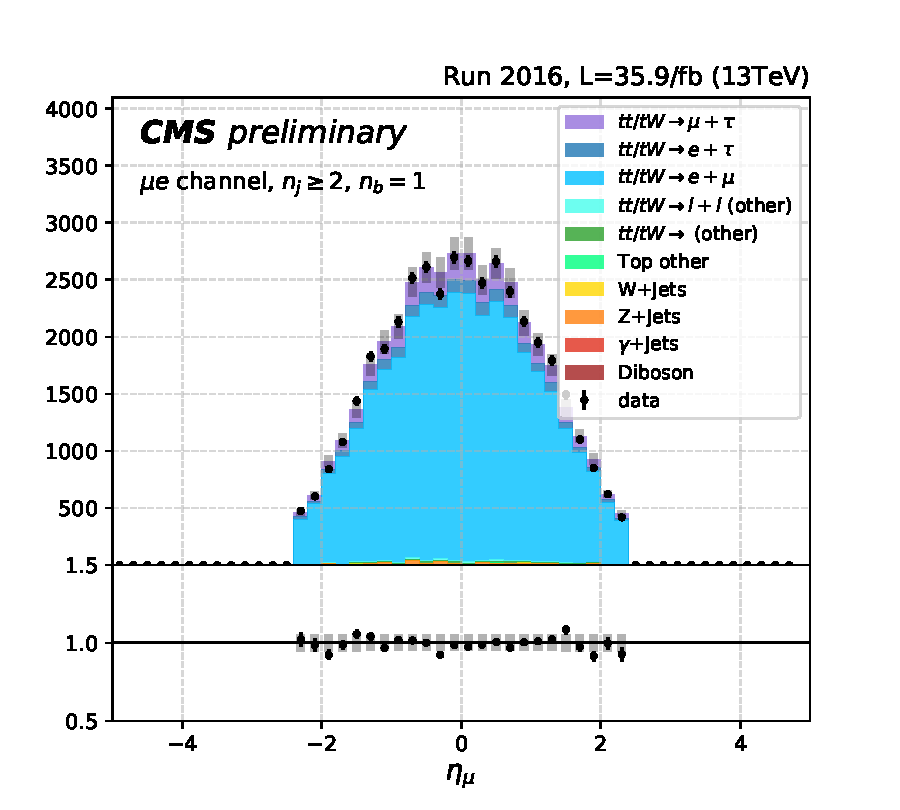
\includegraphics[width=0.49\textwidth]{chapters/Analysis/sectionPlots/figures/kinematics_pickles/emu/1b/emu_1b_lepton1_eta.pdf}
    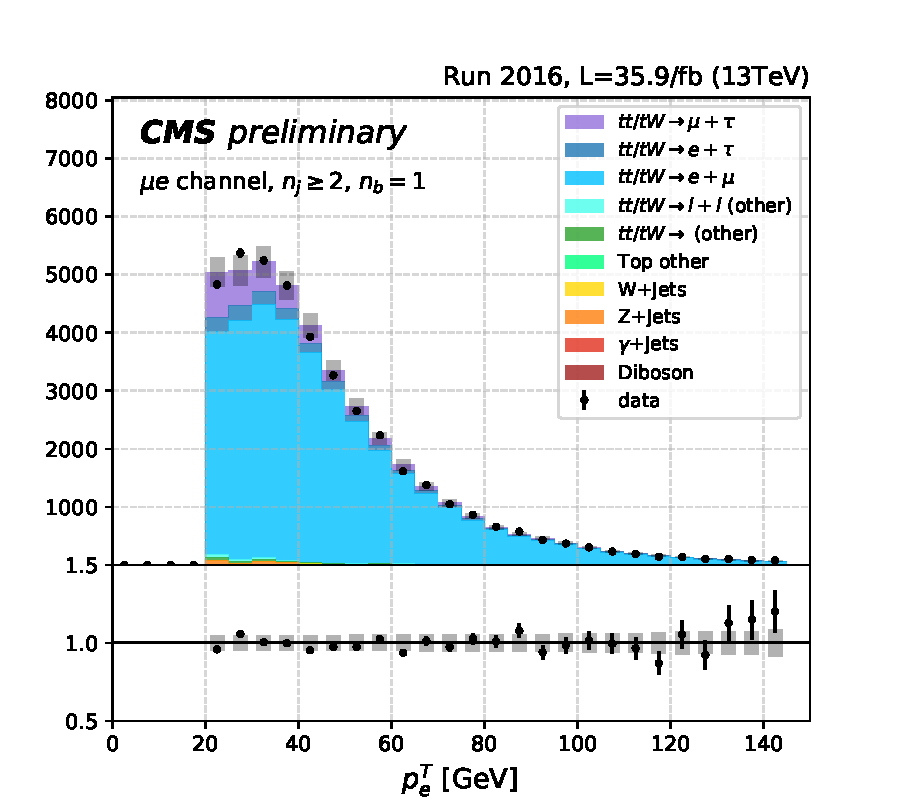
\includegraphics[width=0.49\textwidth]{chapters/Analysis/sectionPlots/figures/kinematics_pickles/emu/1b/emu_1b_lepton2_pt.pdf}
    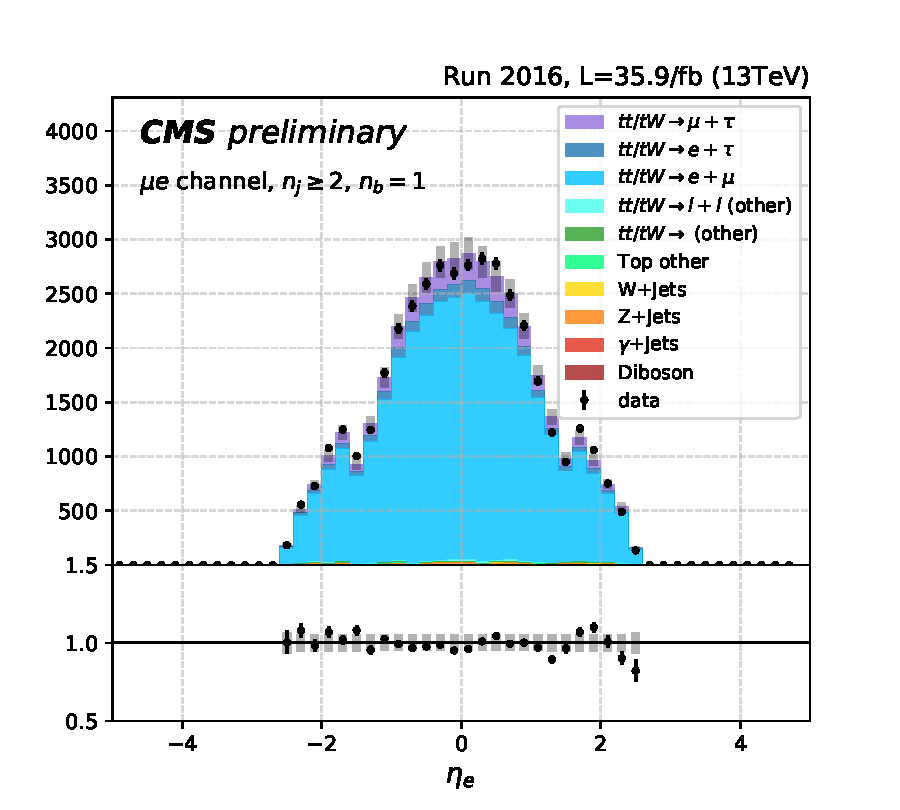
\includegraphics[width=0.49\textwidth]{chapters/Analysis/sectionPlots/figures/kinematics_pickles/emu/1b/emu_1b_lepton2_eta.pdf}
    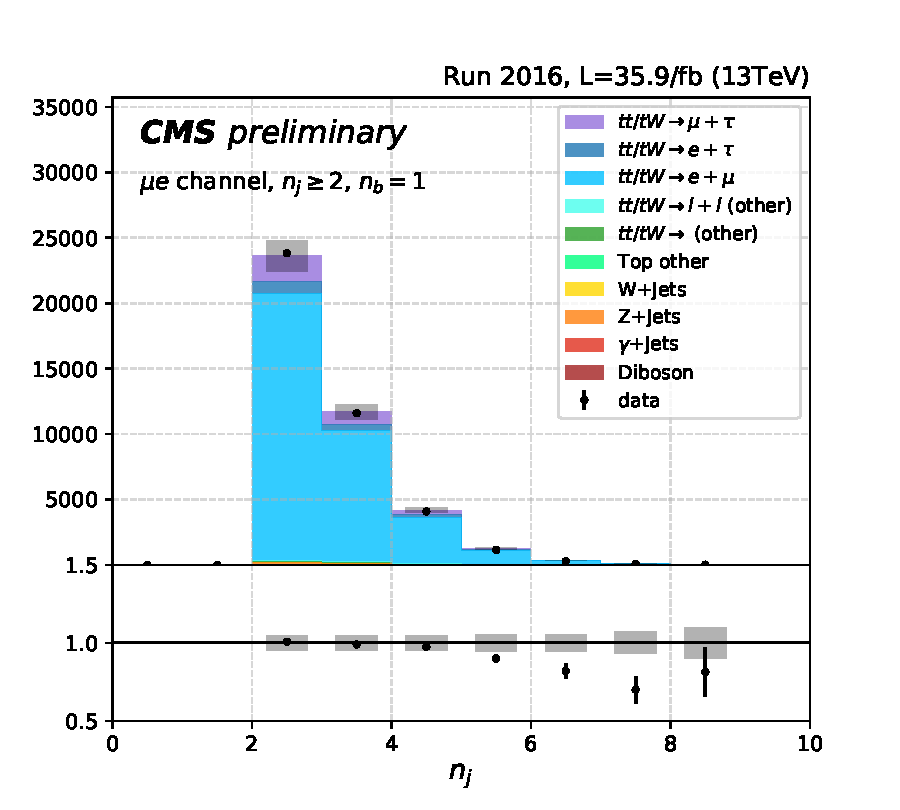
\includegraphics[width=0.49\textwidth]{chapters/Analysis/sectionPlots/figures/kinematics_pickles/emu/1b/emu_1b_nJets.pdf}
    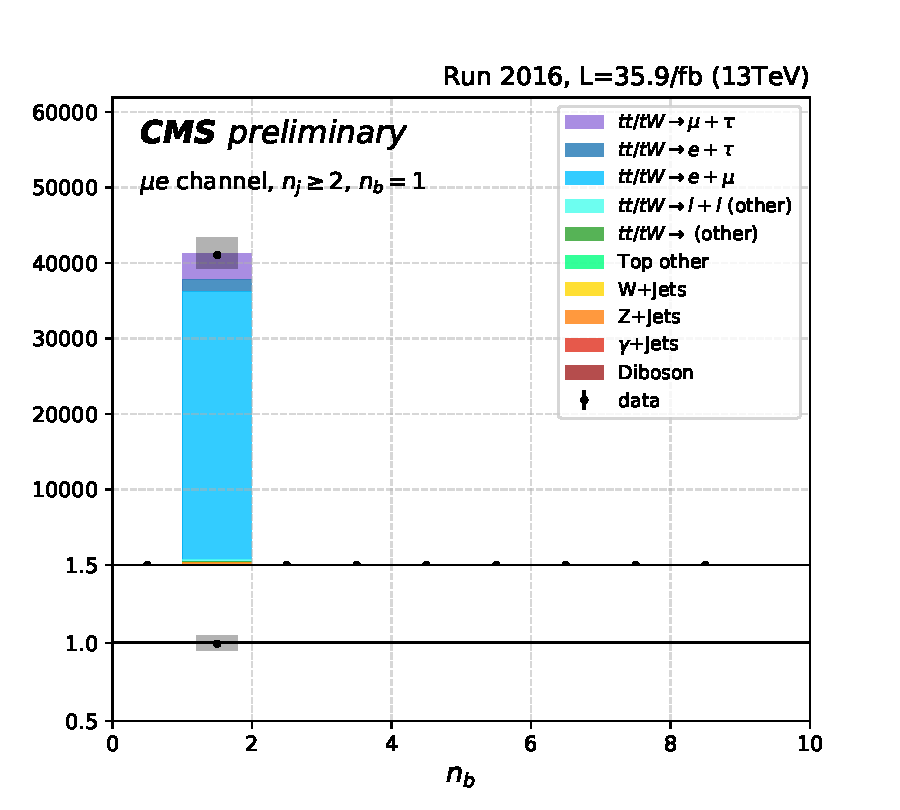
\includegraphics[width=0.49\textwidth]{chapters/Analysis/sectionPlots/figures/kinematics_pickles/emu/1b/emu_1b_nBJets.pdf}
    
    \caption{$\mu e$ channel with $n_j\geq2, n_b=1$.}
\end{figure}

\begin{figure}[ht]
    \centering
    $ \mu e- 2b$ \\
    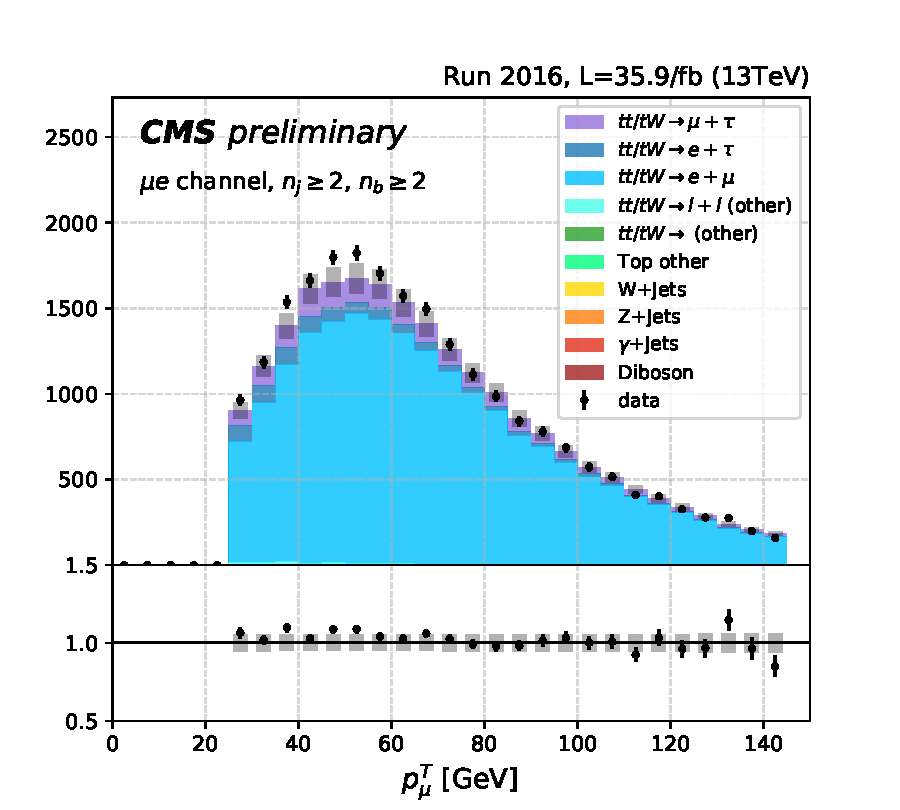
\includegraphics[width=0.49\textwidth]{chapters/Analysis/sectionPlots/figures/kinematics_pickles/emu/2b/emu_2b_lepton1_pt.pdf}
    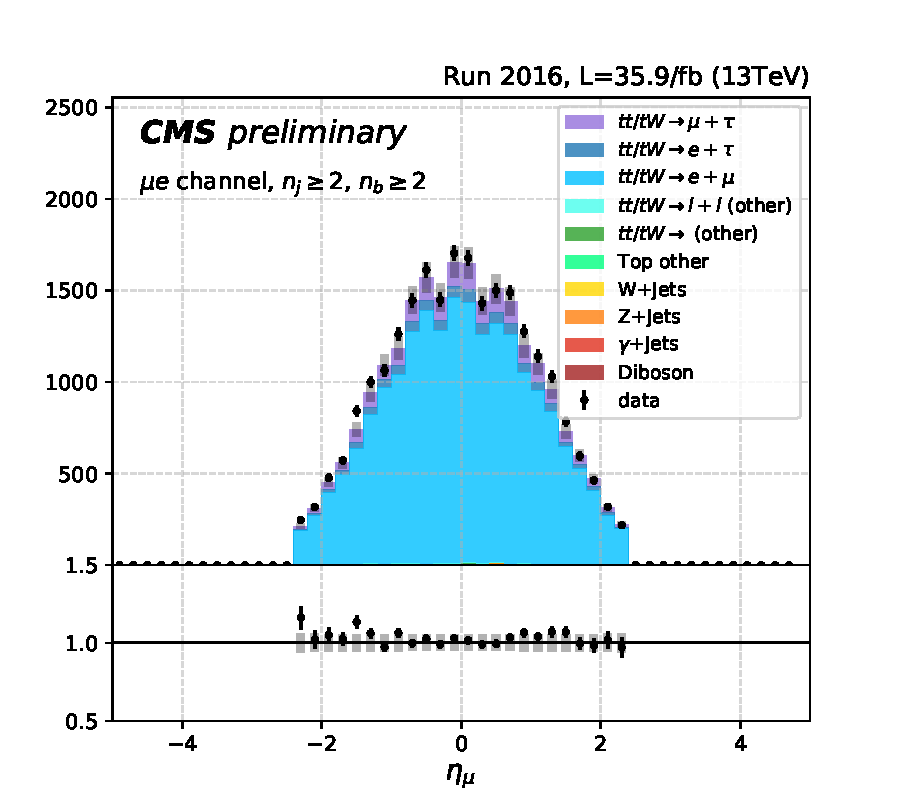
\includegraphics[width=0.49\textwidth]{chapters/Analysis/sectionPlots/figures/kinematics_pickles/emu/2b/emu_2b_lepton1_eta.pdf}
    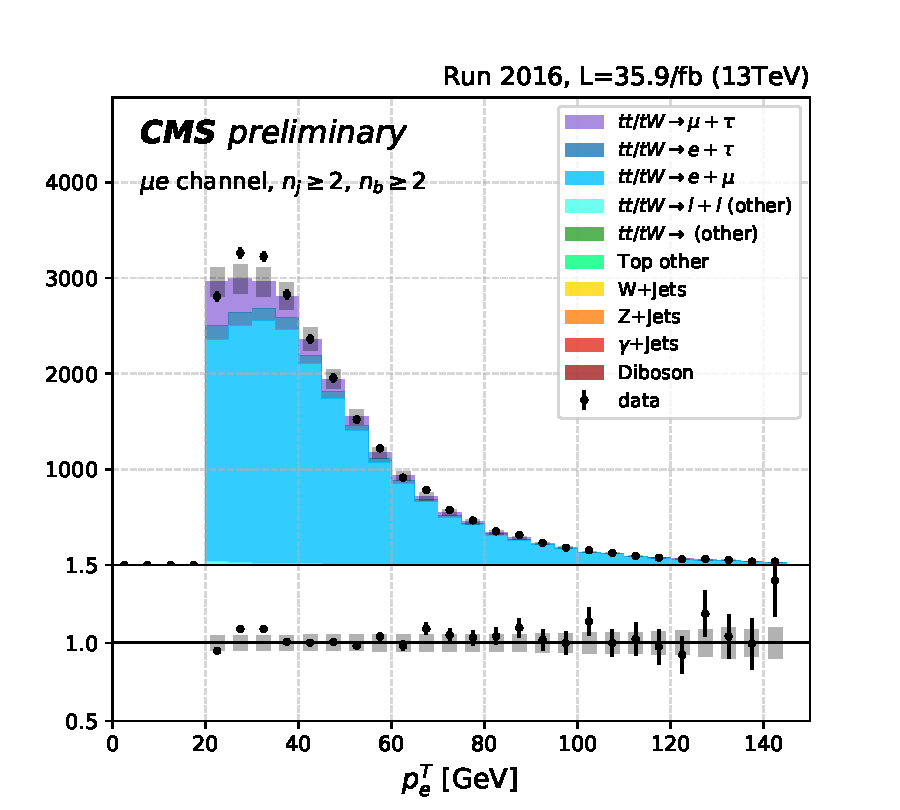
\includegraphics[width=0.49\textwidth]{chapters/Analysis/sectionPlots/figures/kinematics_pickles/emu/2b/emu_2b_lepton2_pt.pdf}
    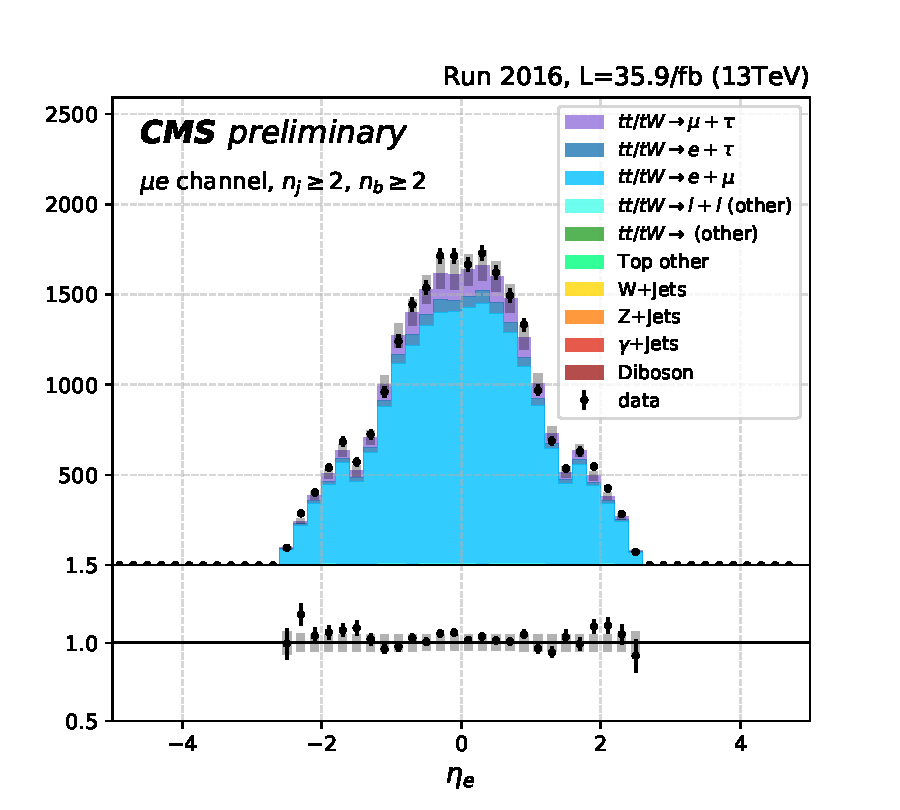
\includegraphics[width=0.49\textwidth]{chapters/Analysis/sectionPlots/figures/kinematics_pickles/emu/2b/emu_2b_lepton2_eta.pdf}
    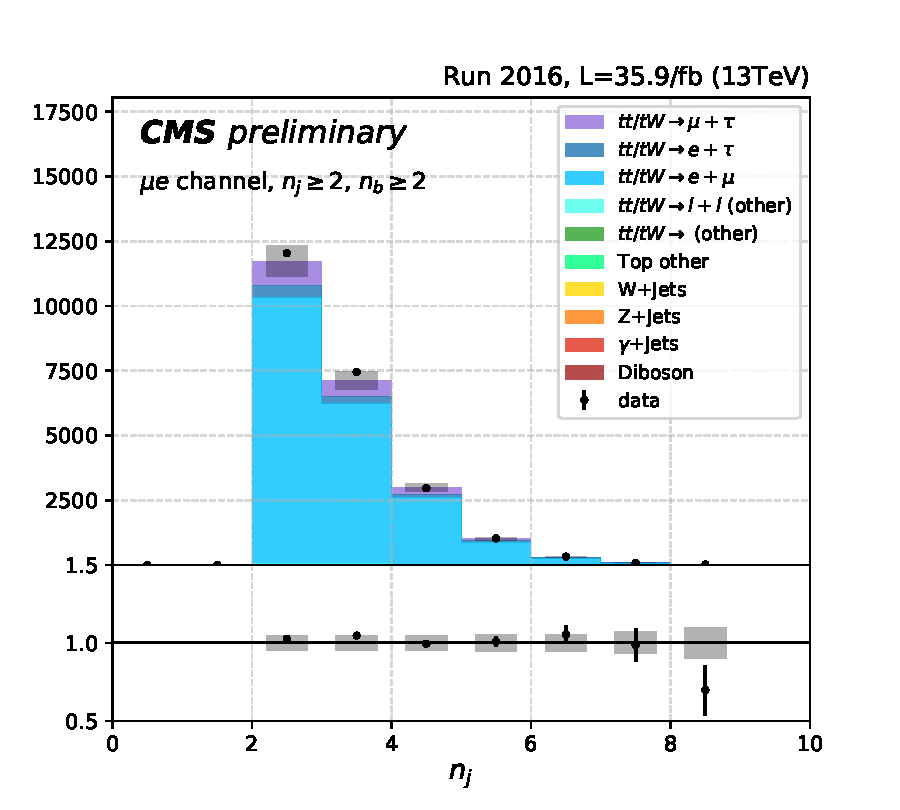
\includegraphics[width=0.49\textwidth]{chapters/Analysis/sectionPlots/figures/kinematics_pickles/emu/2b/emu_2b_nJets.pdf}
    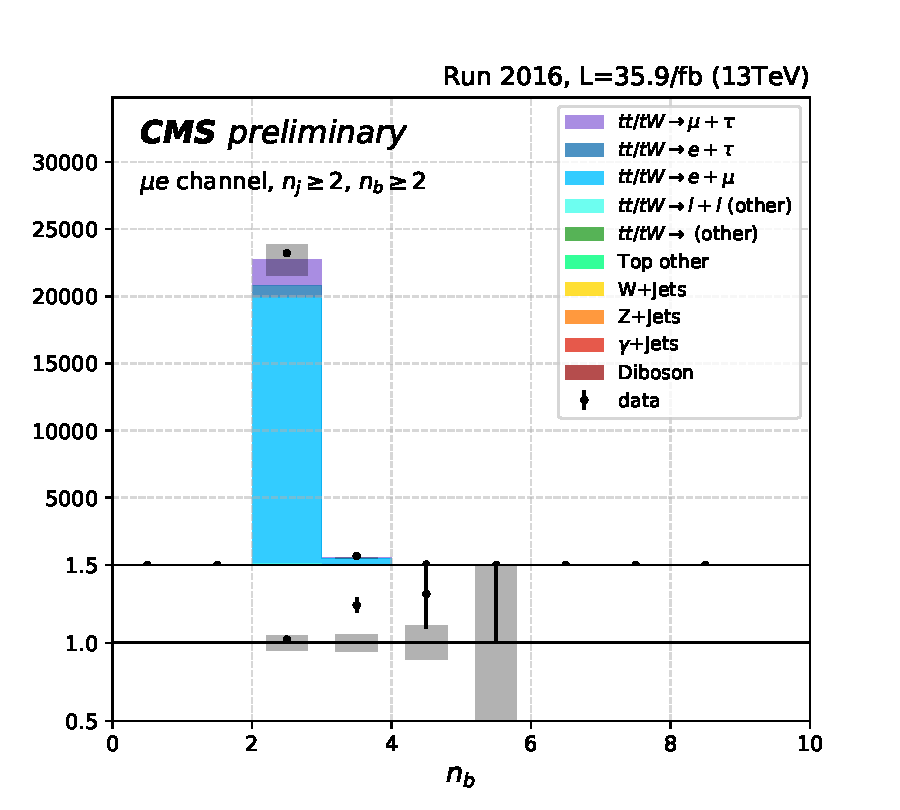
\includegraphics[width=0.49\textwidth]{chapters/Analysis/sectionPlots/figures/kinematics_pickles/emu/2b/emu_2b_nBJets.pdf}
    
    \caption{$\mu e$ channel with $n_j\geq2, n_b\geq2$.}
\end{figure}

%  mumu channel
\begin{figure}[ht]
    \centering
    $\mu\mu - 1b$ \\
    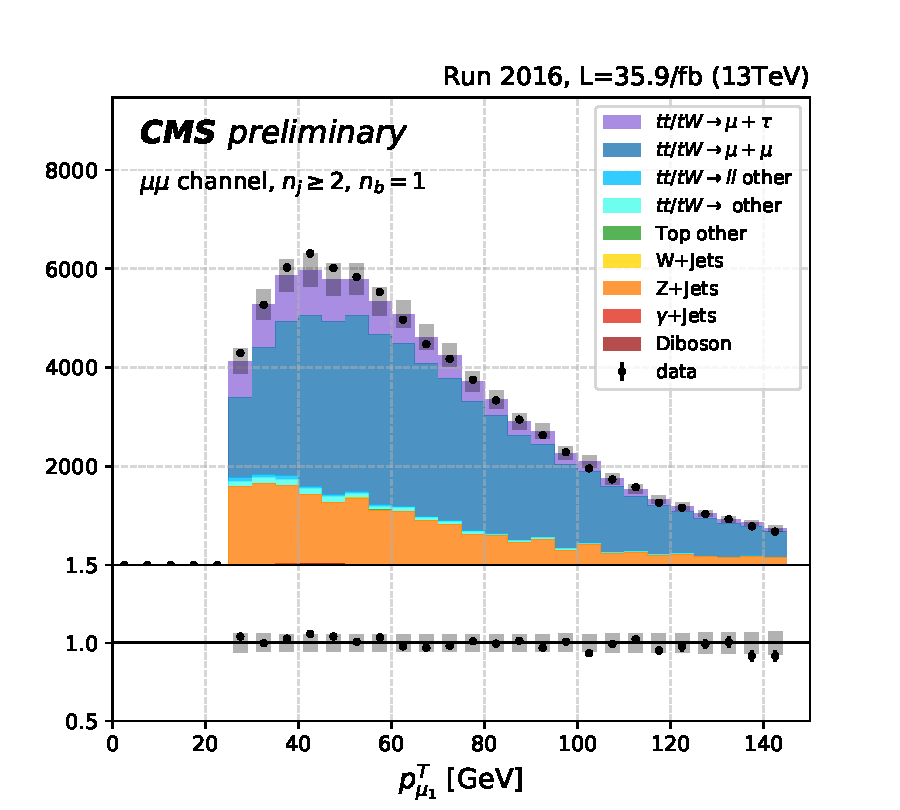
\includegraphics[width=0.49\textwidth]{chapters/Analysis/sectionPlots/figures/kinematics_pickles/mumu/1b/mumu_1b_lepton1_pt.pdf}
    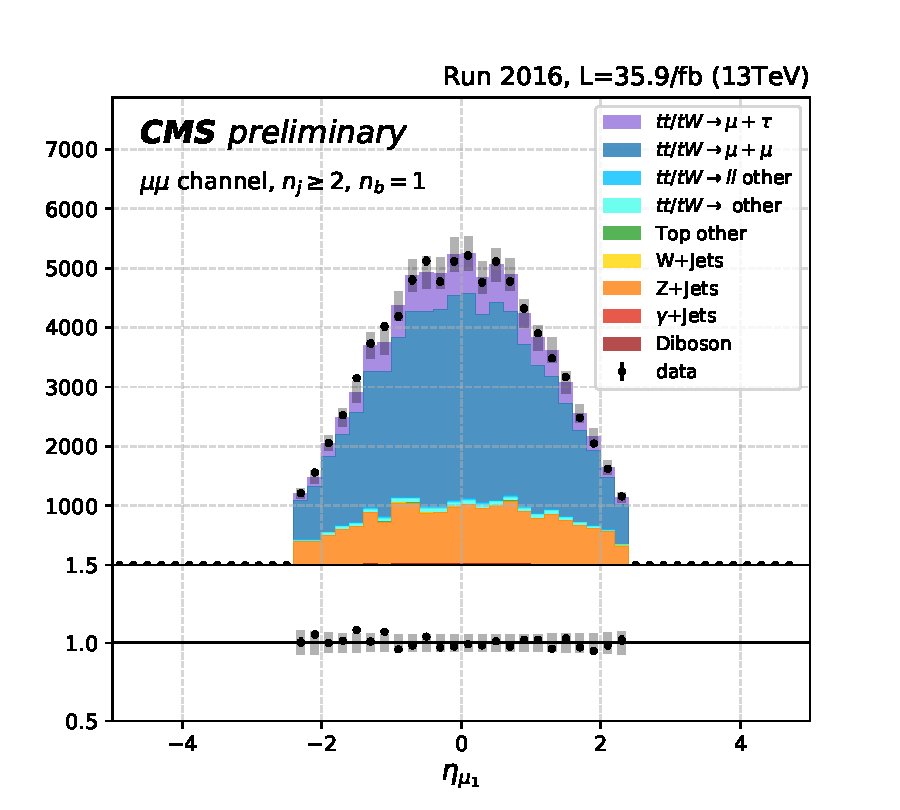
\includegraphics[width=0.49\textwidth]{chapters/Analysis/sectionPlots/figures/kinematics_pickles/mumu/1b/mumu_1b_lepton1_eta.pdf}
    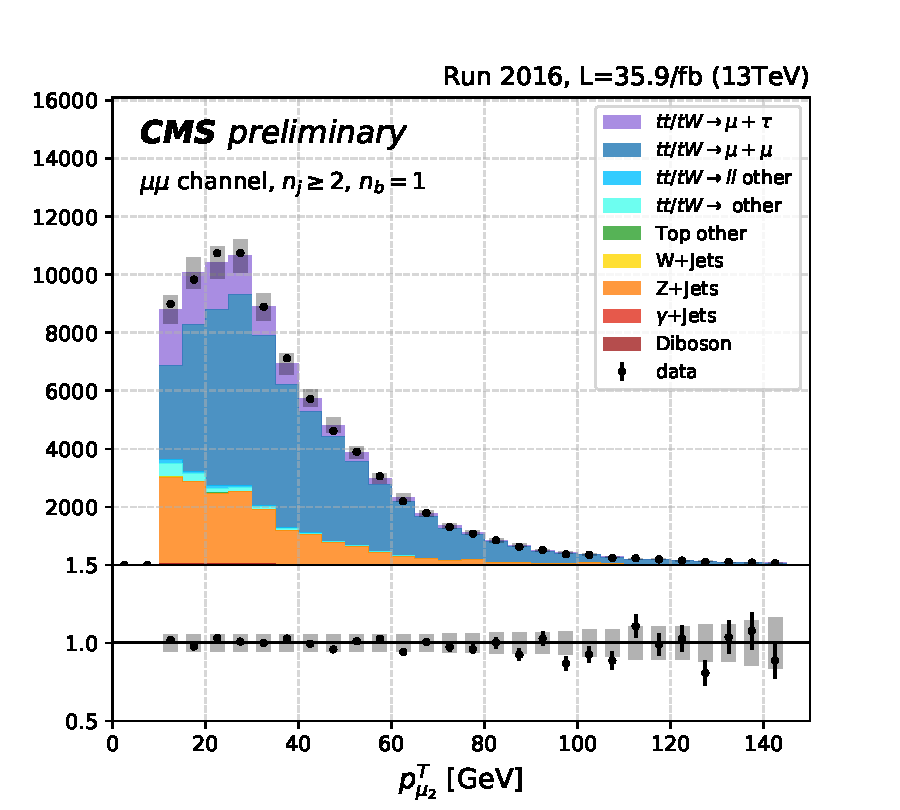
\includegraphics[width=0.49\textwidth]{chapters/Analysis/sectionPlots/figures/kinematics_pickles/mumu/1b/mumu_1b_lepton2_pt.pdf}
    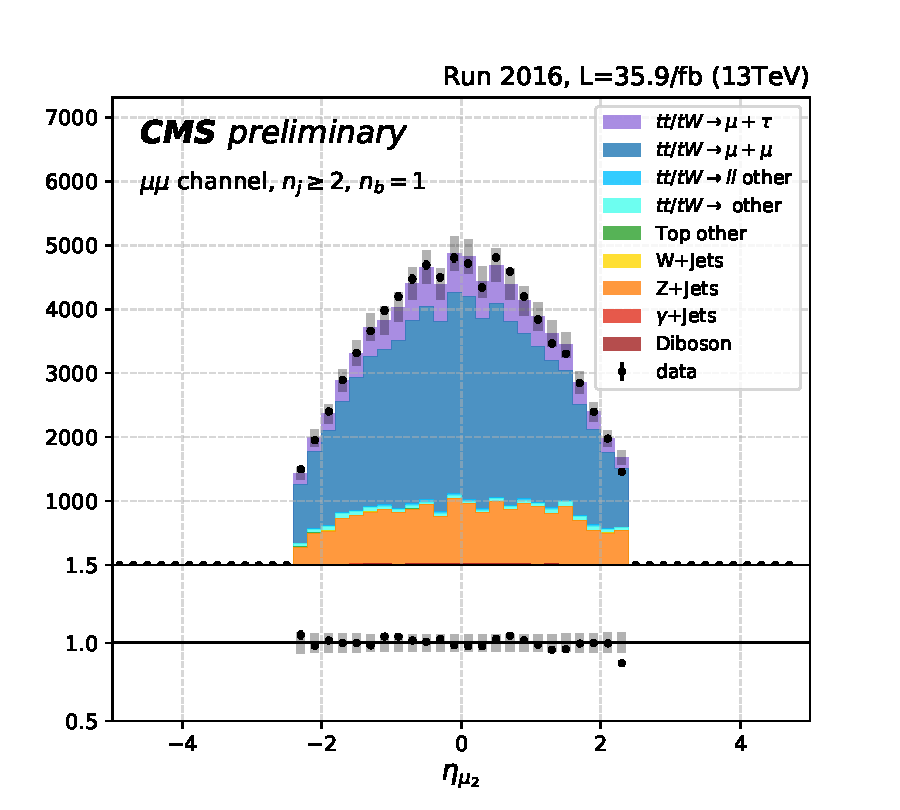
\includegraphics[width=0.49\textwidth]{chapters/Analysis/sectionPlots/figures/kinematics_pickles/mumu/1b/mumu_1b_lepton2_eta.pdf}
    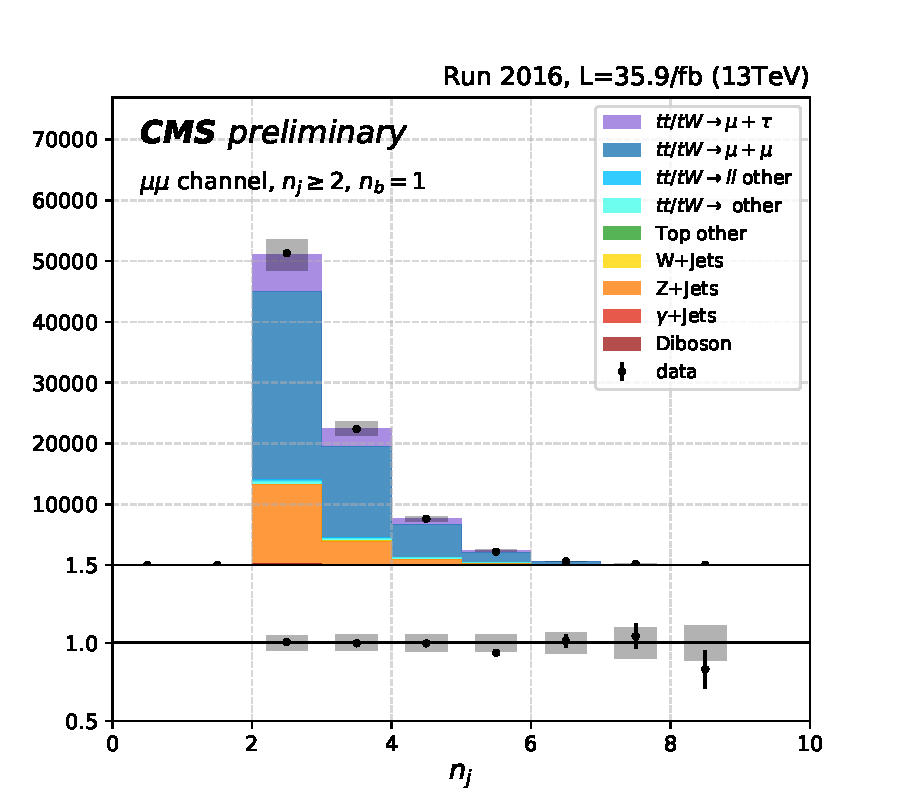
\includegraphics[width=0.49\textwidth]{chapters/Analysis/sectionPlots/figures/kinematics_pickles/mumu/1b/mumu_1b_nJets.pdf}
    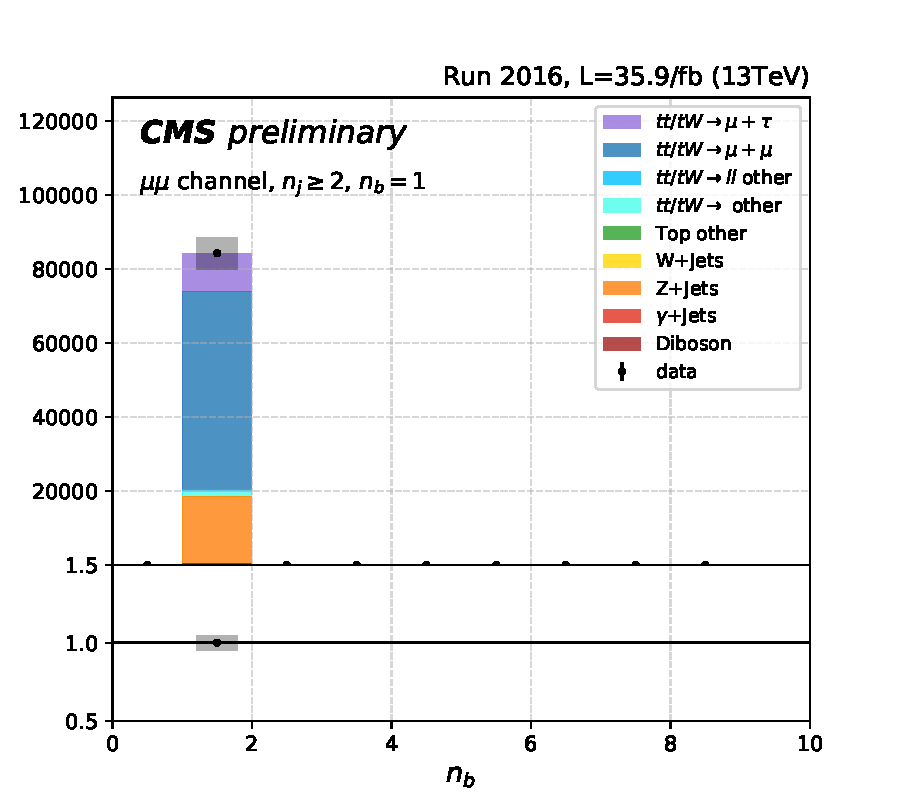
\includegraphics[width=0.49\textwidth]{chapters/Analysis/sectionPlots/figures/kinematics_pickles/mumu/1b/mumu_1b_nBJets.pdf}
    
    \caption{$\mu \mu$ channel with $n_j\geq2, n_b=1$.}
\end{figure}

\begin{figure}[ht]
    \centering
    $\mu\mu - 2b$ \\
    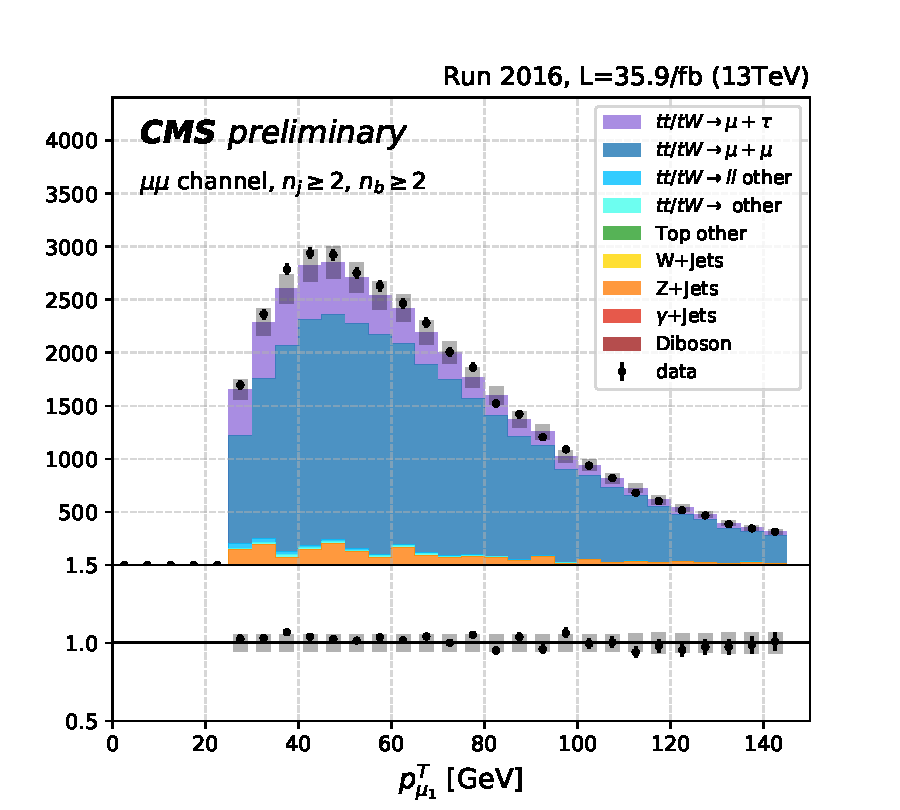
\includegraphics[width=0.49\textwidth]{chapters/Analysis/sectionPlots/figures/kinematics_pickles/mumu/2b/mumu_2b_lepton1_pt.pdf}
    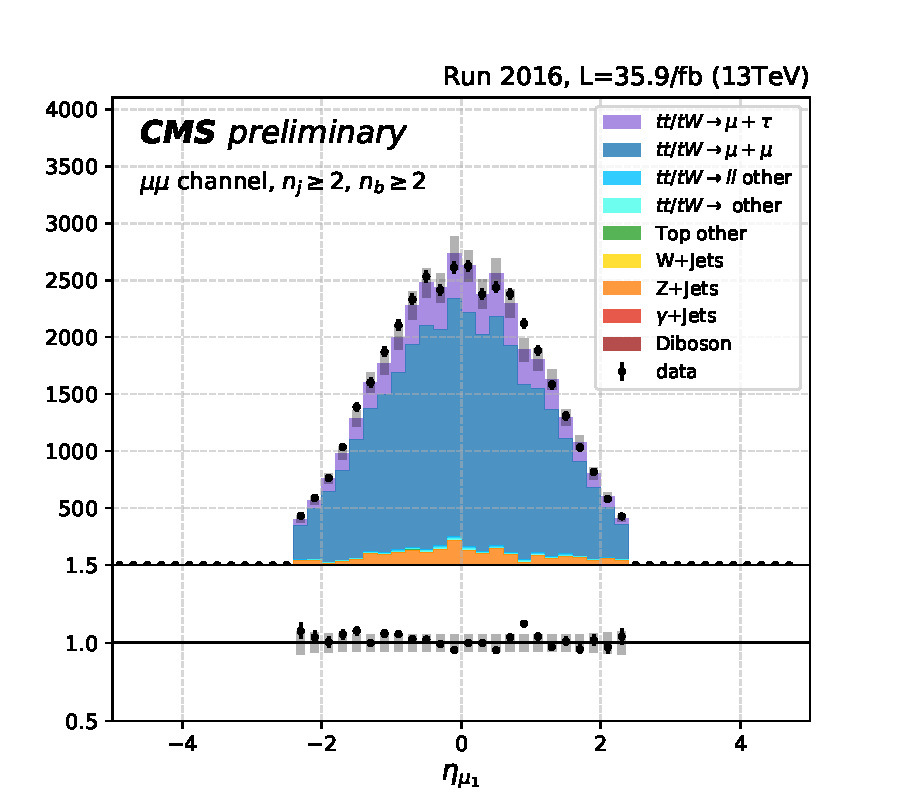
\includegraphics[width=0.49\textwidth]{chapters/Analysis/sectionPlots/figures/kinematics_pickles/mumu/2b/mumu_2b_lepton1_eta.pdf}
    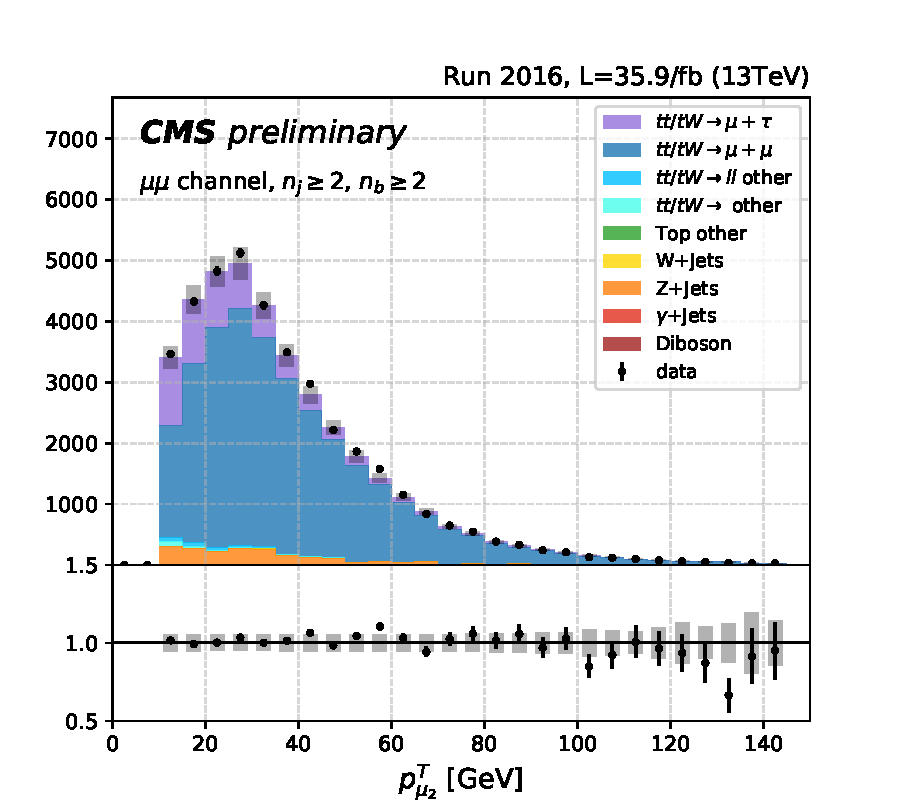
\includegraphics[width=0.49\textwidth]{chapters/Analysis/sectionPlots/figures/kinematics_pickles/mumu/2b/mumu_2b_lepton2_pt.pdf}
    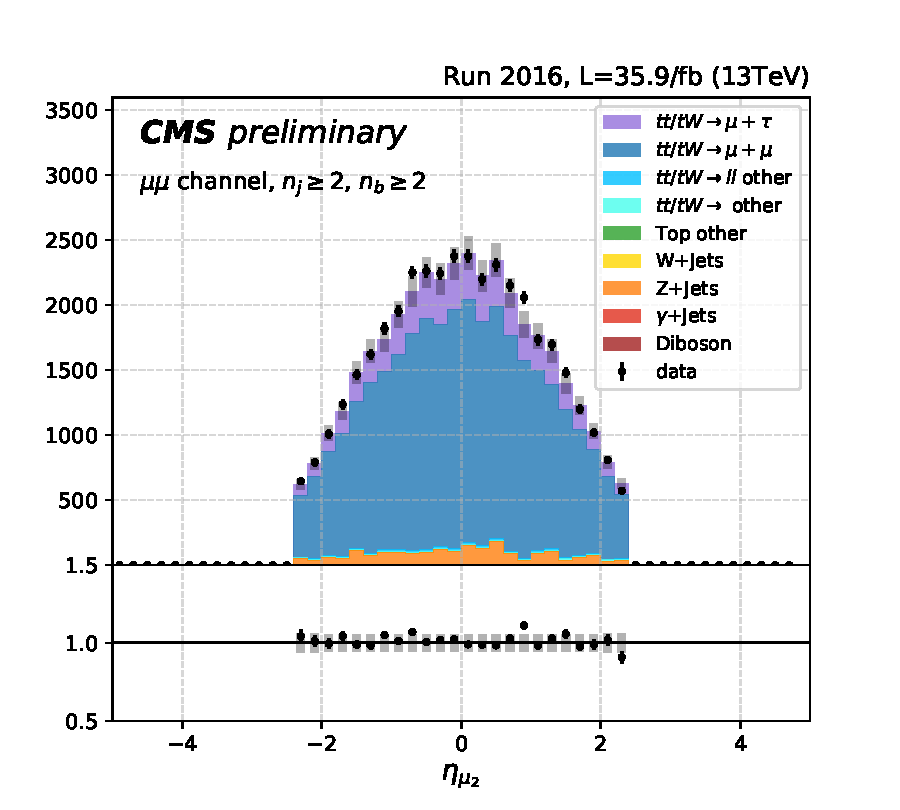
\includegraphics[width=0.49\textwidth]{chapters/Analysis/sectionPlots/figures/kinematics_pickles/mumu/2b/mumu_2b_lepton2_eta.pdf}
    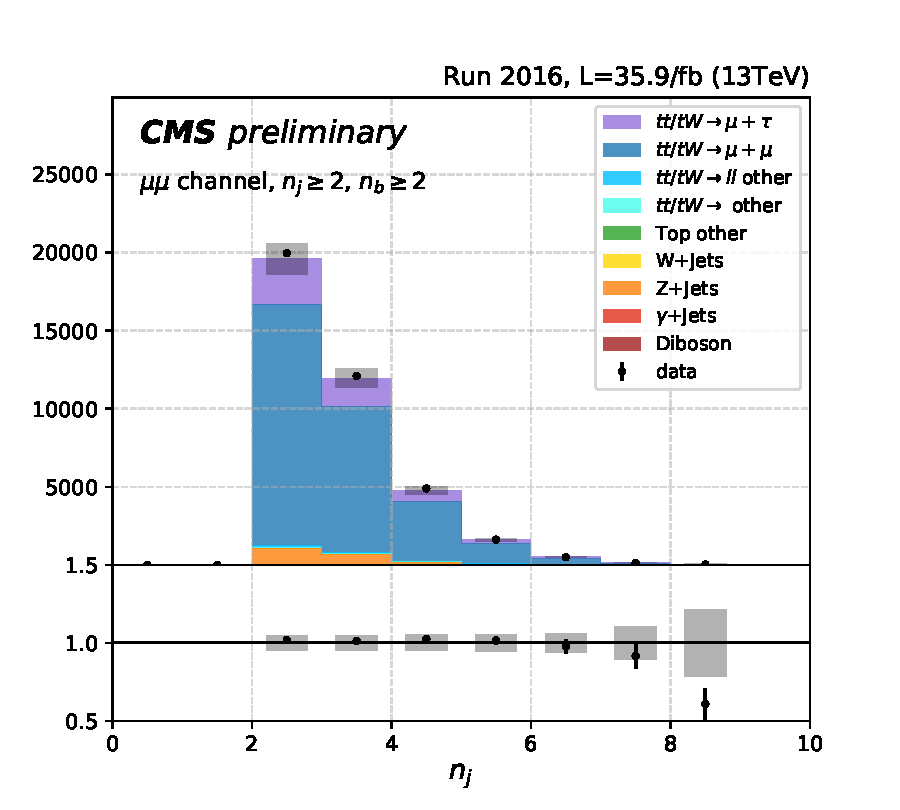
\includegraphics[width=0.49\textwidth]{chapters/Analysis/sectionPlots/figures/kinematics_pickles/mumu/2b/mumu_2b_nJets.pdf}
    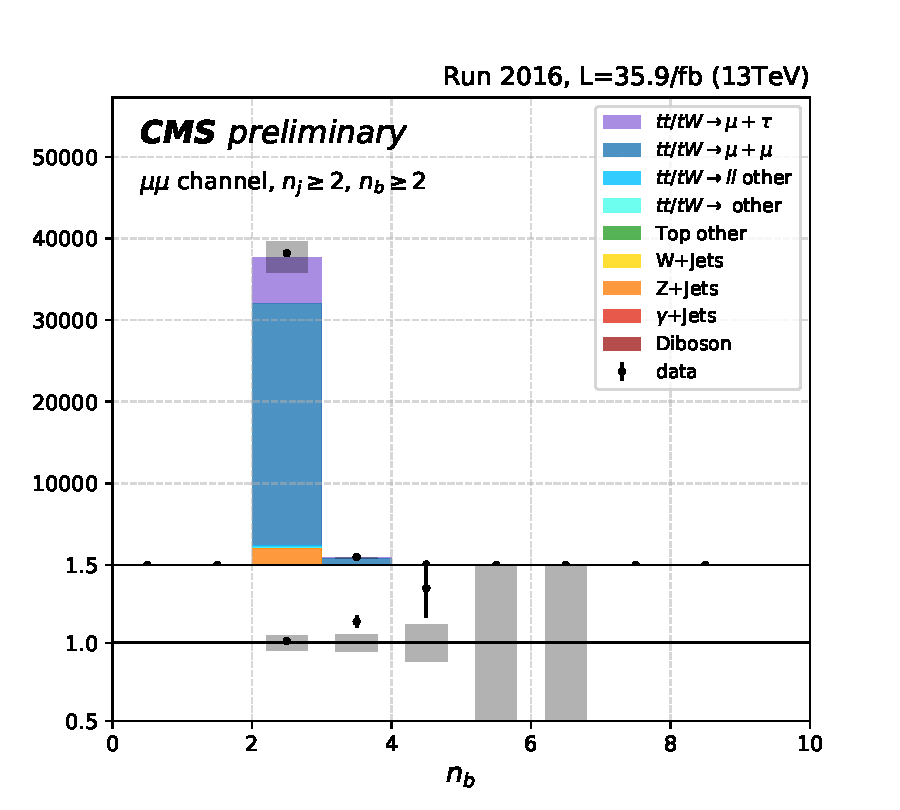
\includegraphics[width=0.49\textwidth]{chapters/Analysis/sectionPlots/figures/kinematics_pickles/mumu/2b/mumu_2b_nBJets.pdf}
    
    \caption{$\mu\mu$ channel with $n_j\geq2, n_b\geq2$.}
\end{figure}


%  mutau channel
\begin{figure}[ht]
    \centering
    $\mu\tau - 1b$ \\
    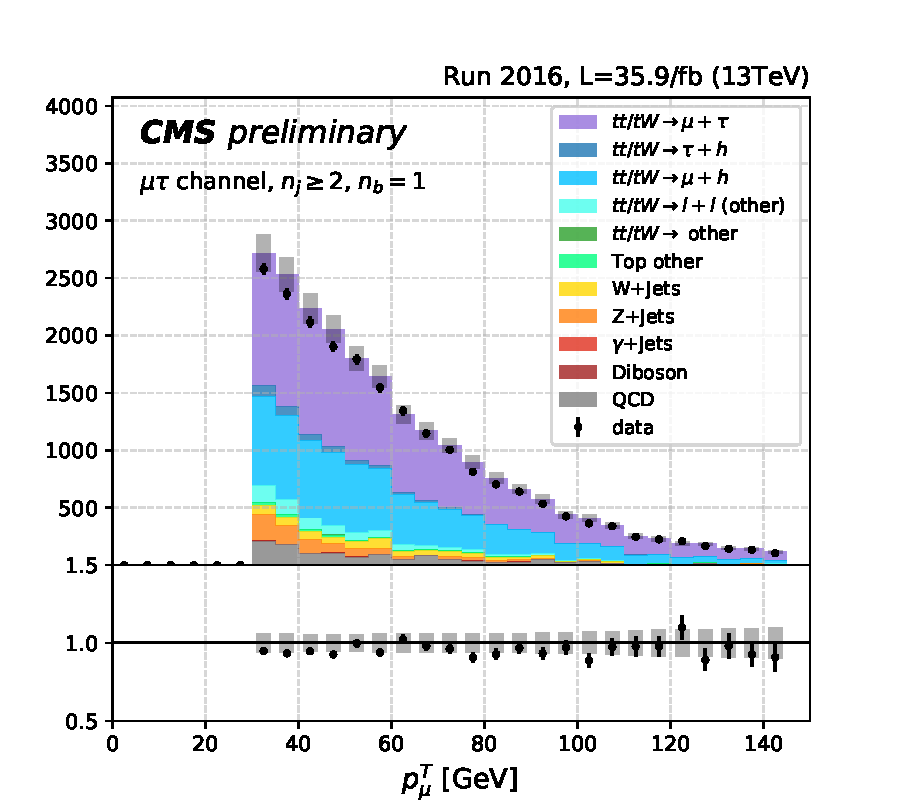
\includegraphics[width=0.49\textwidth]{chapters/Analysis/sectionPlots/figures/kinematics_pickles/mutau/1b/mutau_1b_lepton1_pt.pdf}
    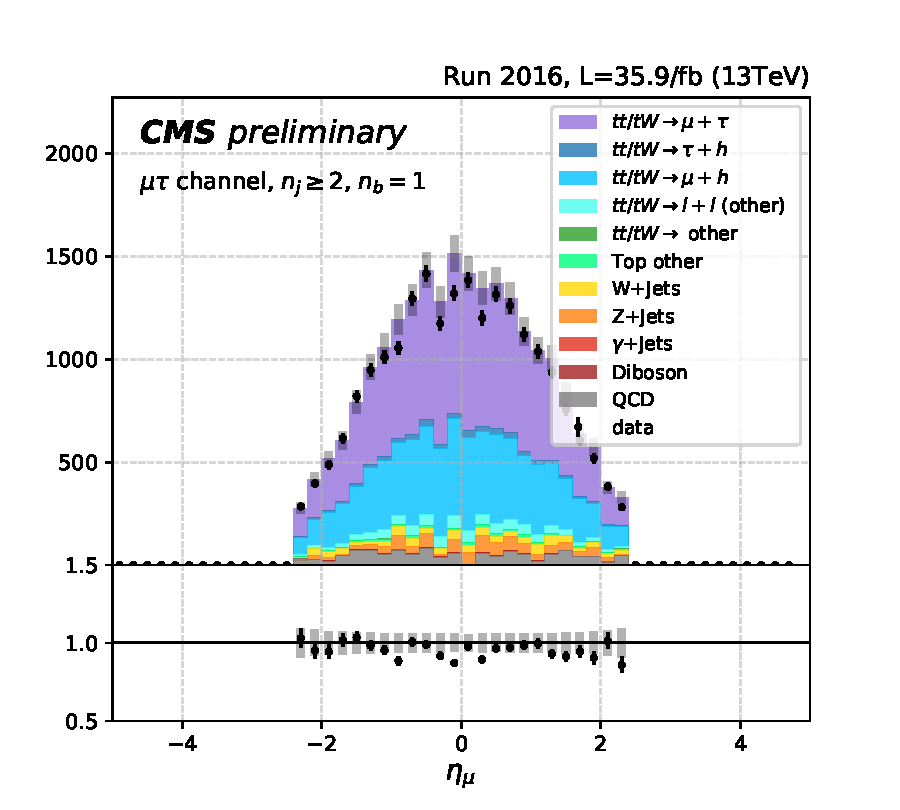
\includegraphics[width=0.49\textwidth]{chapters/Analysis/sectionPlots/figures/kinematics_pickles/mutau/1b/mutau_1b_lepton1_eta.pdf}
    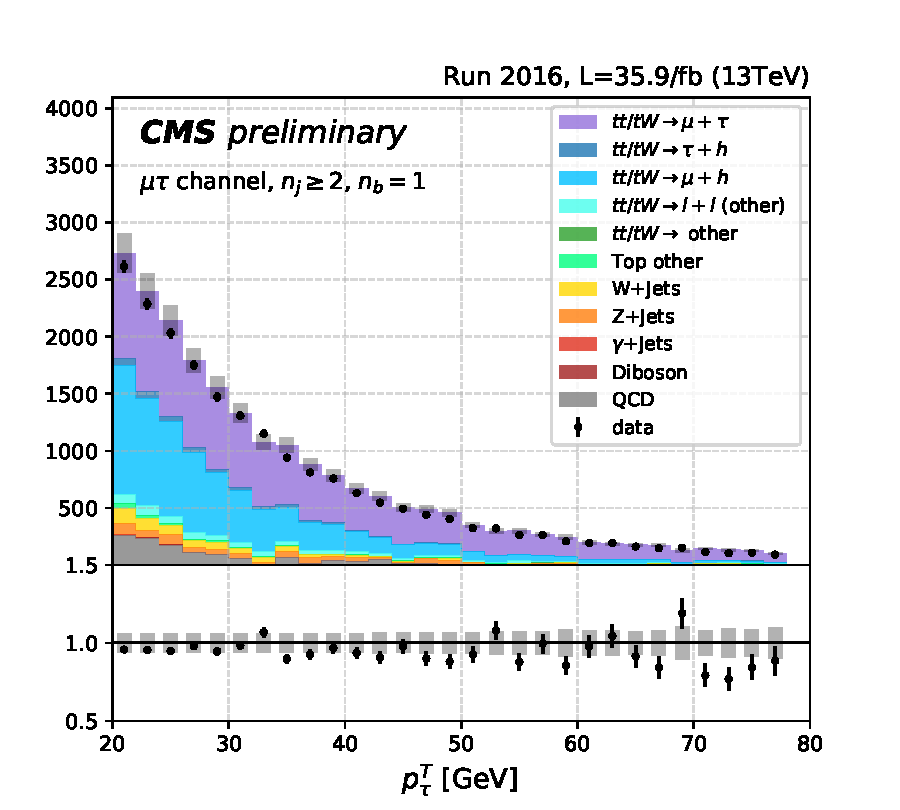
\includegraphics[width=0.49\textwidth]{chapters/Analysis/sectionPlots/figures/kinematics_pickles/mutau/1b/mutau_1b_lepton2_pt.pdf}
    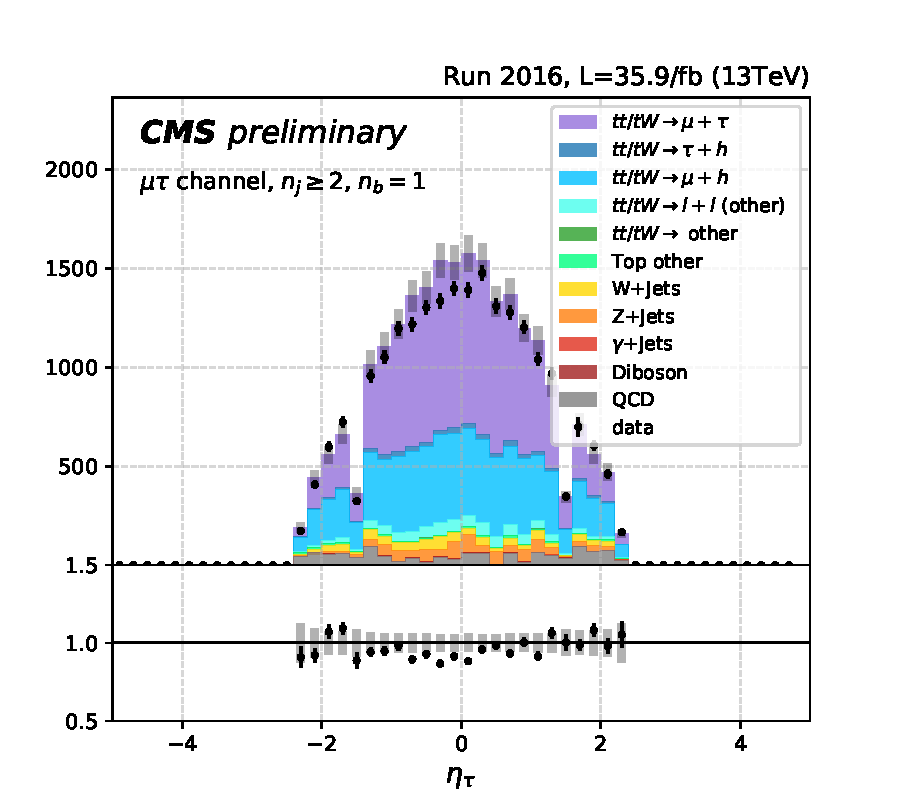
\includegraphics[width=0.49\textwidth]{chapters/Analysis/sectionPlots/figures/kinematics_pickles/mutau/1b/mutau_1b_lepton2_eta.pdf}
    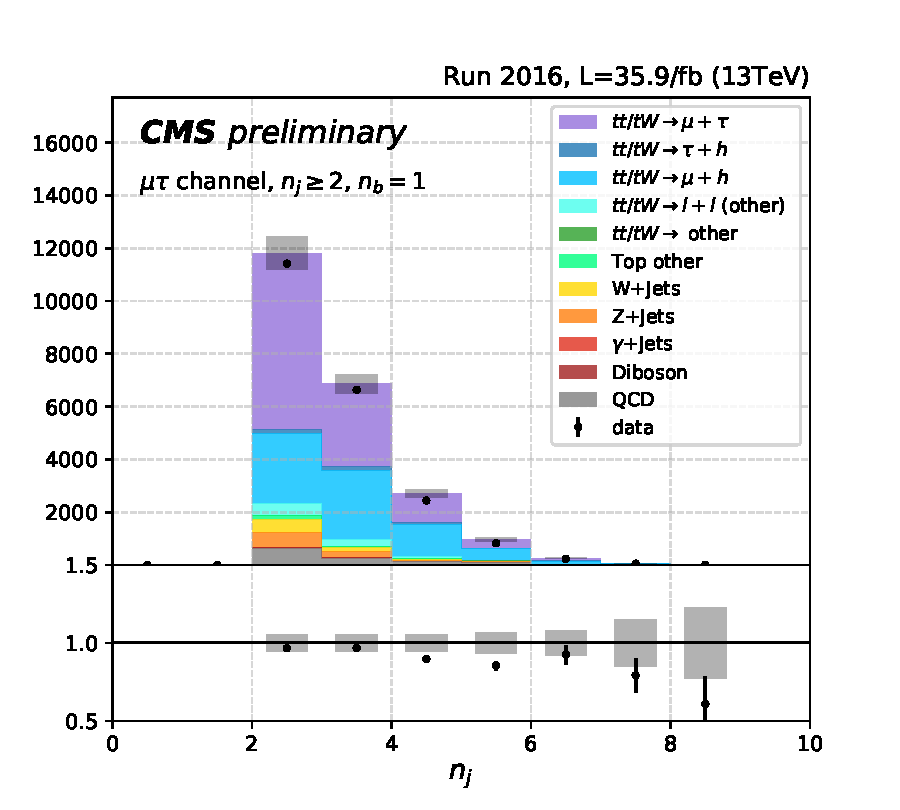
\includegraphics[width=0.49\textwidth]{chapters/Analysis/sectionPlots/figures/kinematics_pickles/mutau/1b/mutau_1b_nJets.pdf}
    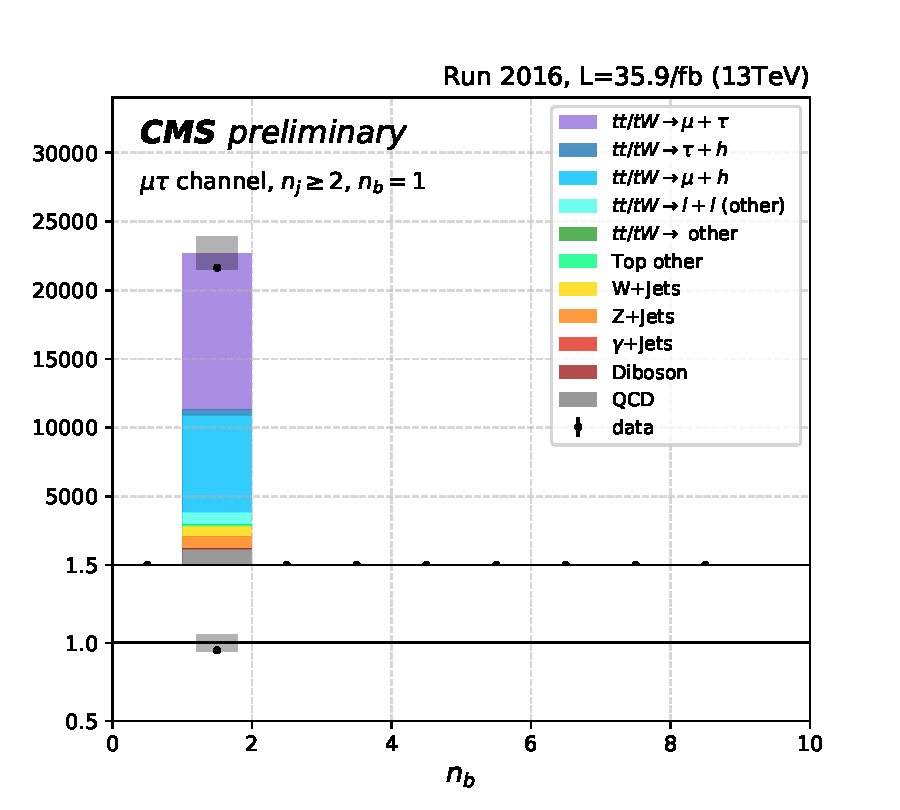
\includegraphics[width=0.49\textwidth]{chapters/Analysis/sectionPlots/figures/kinematics_pickles/mutau/1b/mutau_1b_nBJets.pdf}
    
    \caption{$\mu\tau$ channel with $n_j\geq2, n_b=1$.}
\end{figure}

\begin{figure}[ht]
    \centering
    $\mu\tau - 2b$ \\
    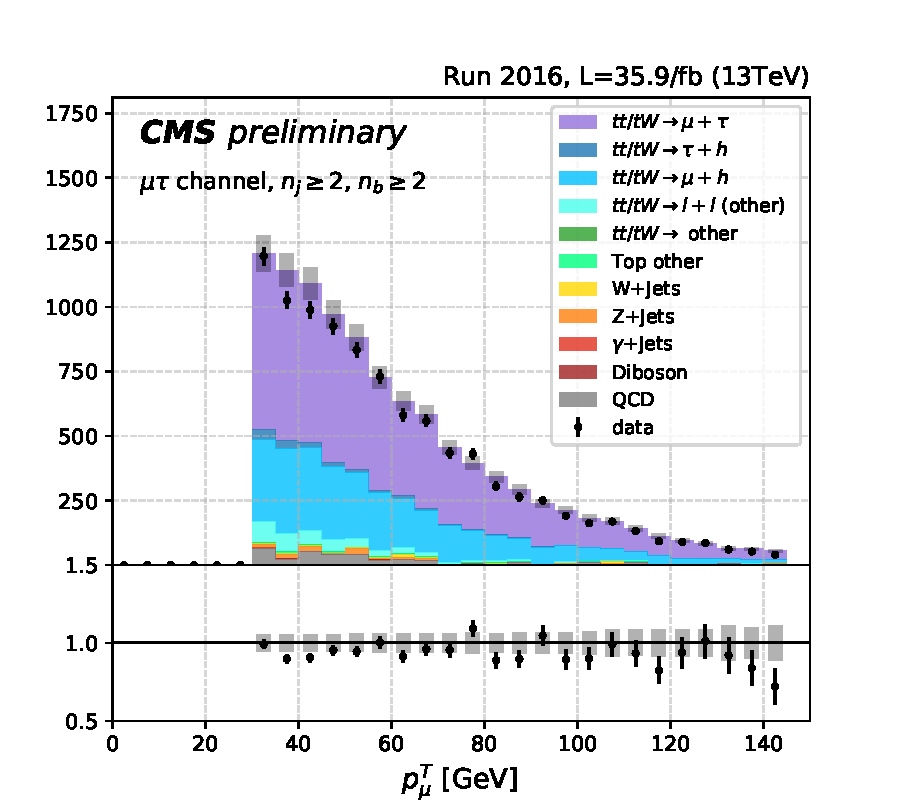
\includegraphics[width=0.49\textwidth]{chapters/Analysis/sectionPlots/figures/kinematics_pickles/mutau/2b/mutau_2b_lepton1_pt.pdf}
    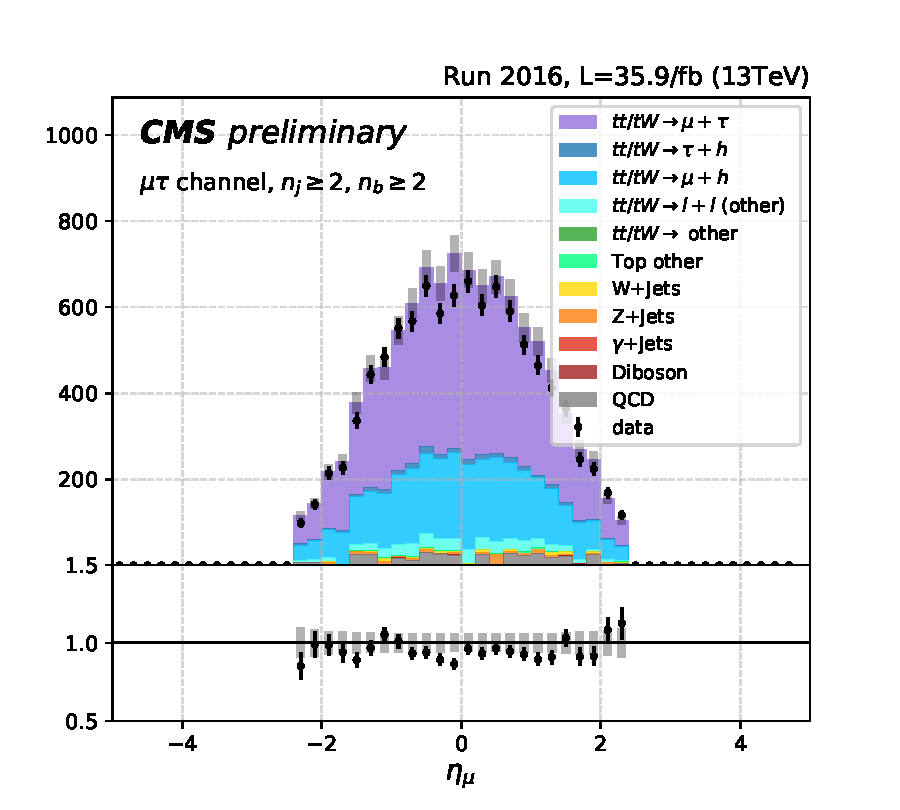
\includegraphics[width=0.49\textwidth]{chapters/Analysis/sectionPlots/figures/kinematics_pickles/mutau/2b/mutau_2b_lepton1_eta.pdf}
    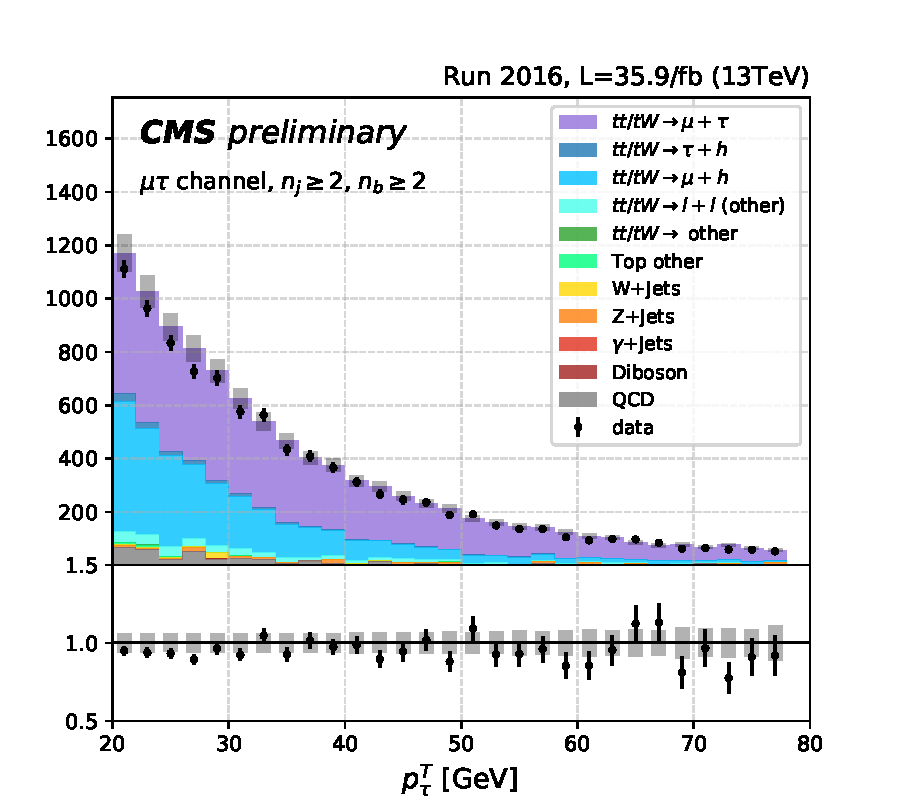
\includegraphics[width=0.49\textwidth]{chapters/Analysis/sectionPlots/figures/kinematics_pickles/mutau/2b/mutau_2b_lepton2_pt.pdf}
    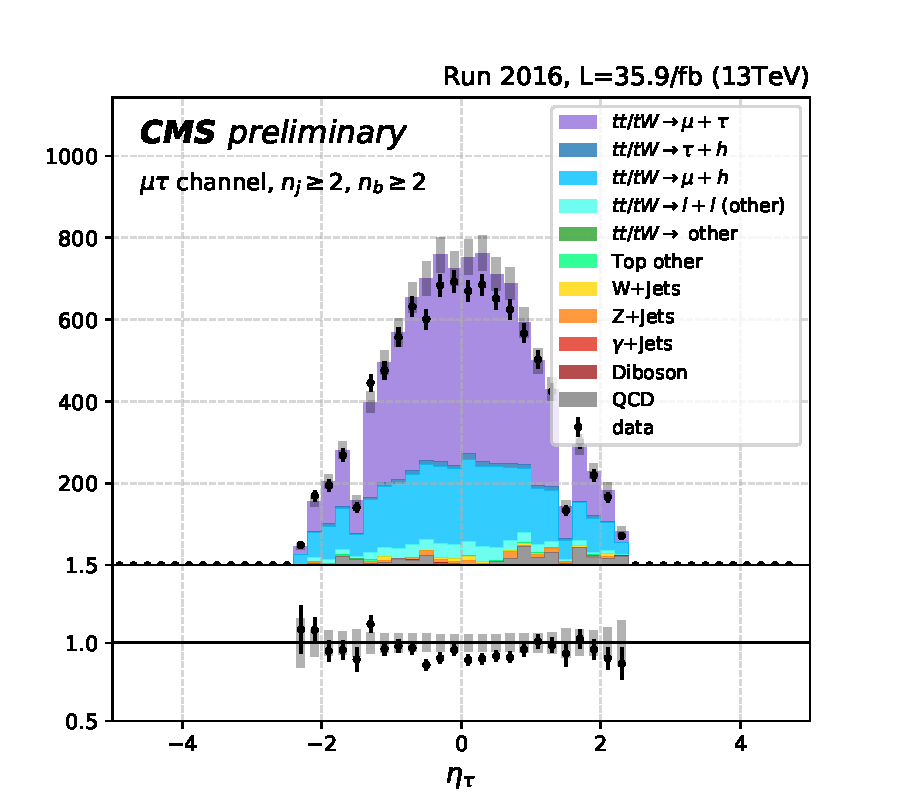
\includegraphics[width=0.49\textwidth]{chapters/Analysis/sectionPlots/figures/kinematics_pickles/mutau/2b/mutau_2b_lepton2_eta.pdf}
    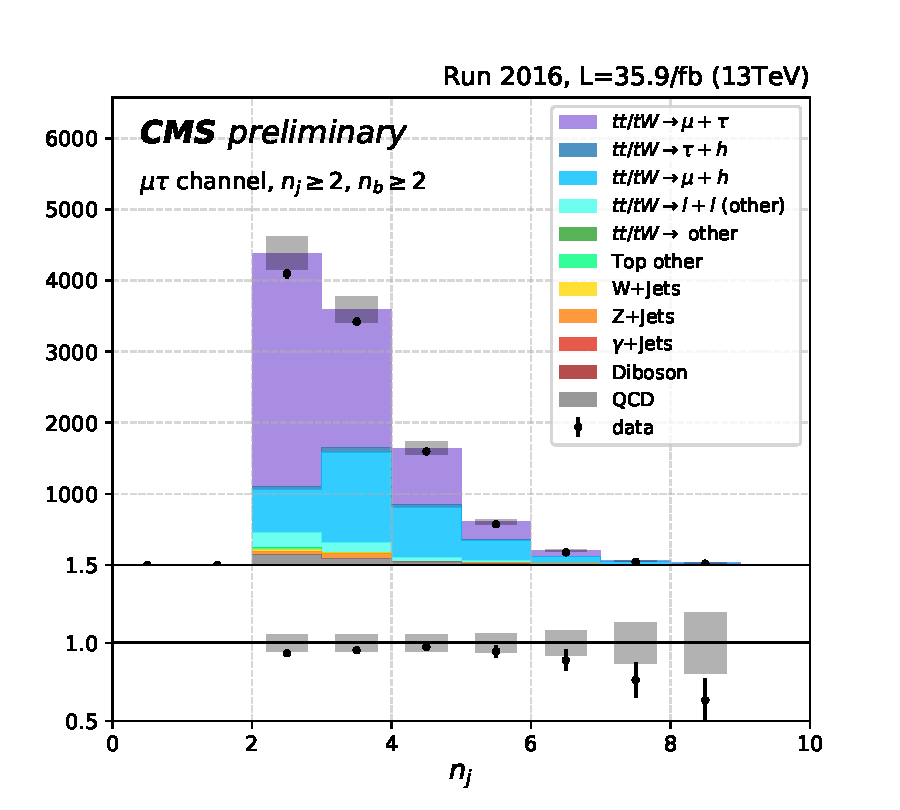
\includegraphics[width=0.49\textwidth]{chapters/Analysis/sectionPlots/figures/kinematics_pickles/mutau/2b/mutau_2b_nJets.pdf}
    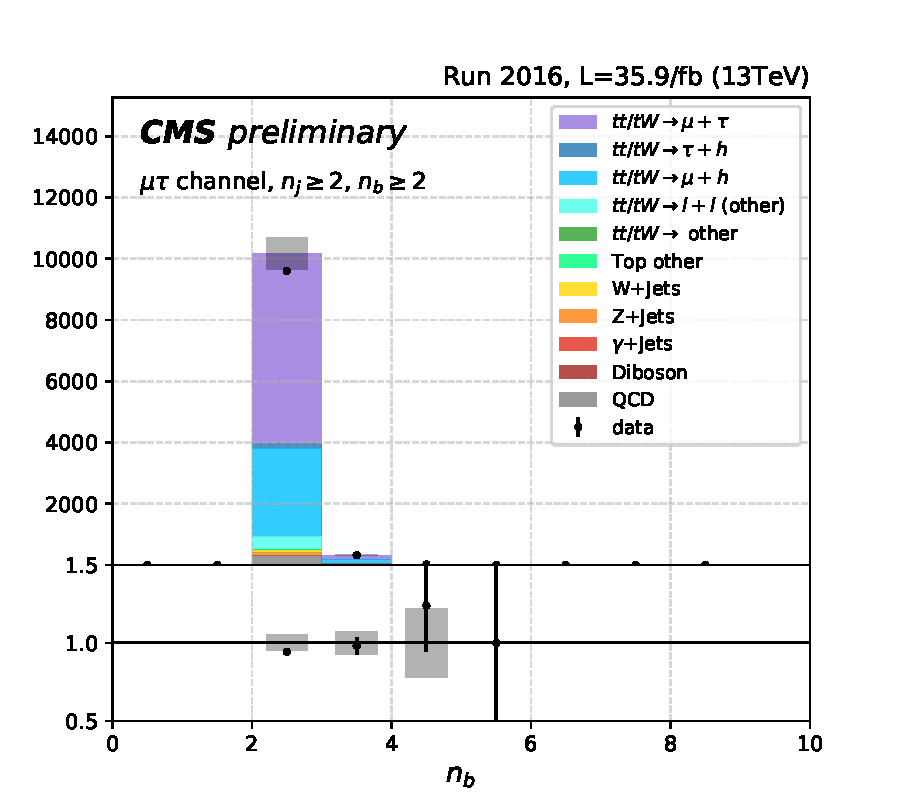
\includegraphics[width=0.49\textwidth]{chapters/Analysis/sectionPlots/figures/kinematics_pickles/mutau/2b/mutau_2b_nBJets.pdf}
    
    \caption{$\mu\tau$ channel with $n_j\geq2, n_b\geq2$.}
\end{figure}


% muj channel
\begin{figure}[ht]
    \centering
    $\mu j- 1b$ \\
    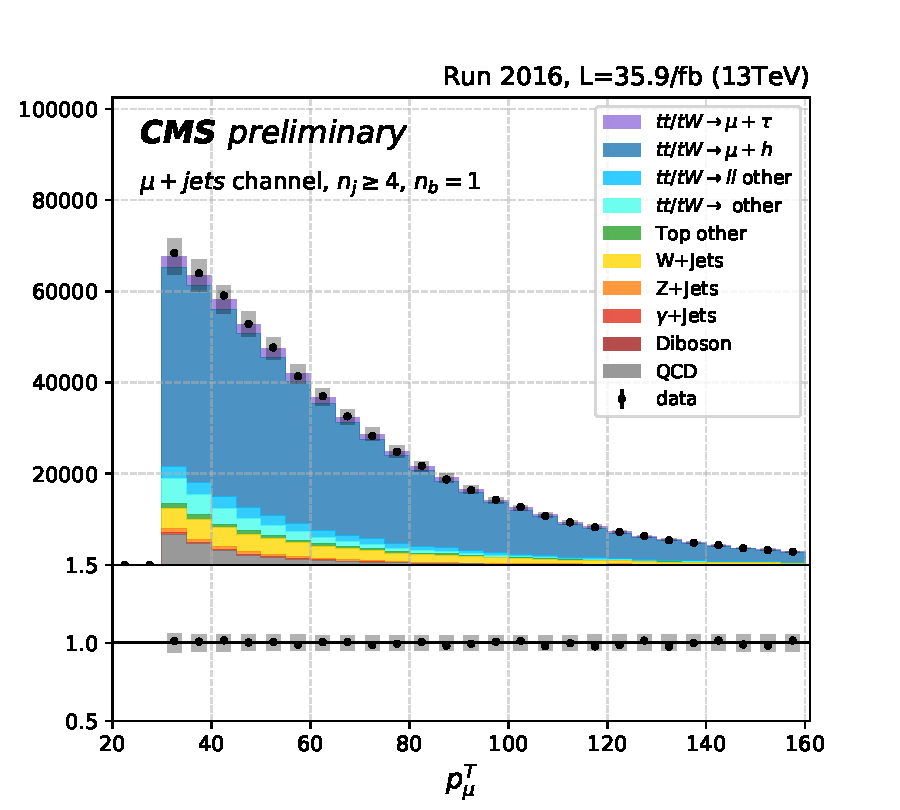
\includegraphics[width=0.49\textwidth]{chapters/Analysis/sectionPlots/figures/kinematics_pickles/mu4j/1b/mu4j_1b_lepton1_pt.pdf}
    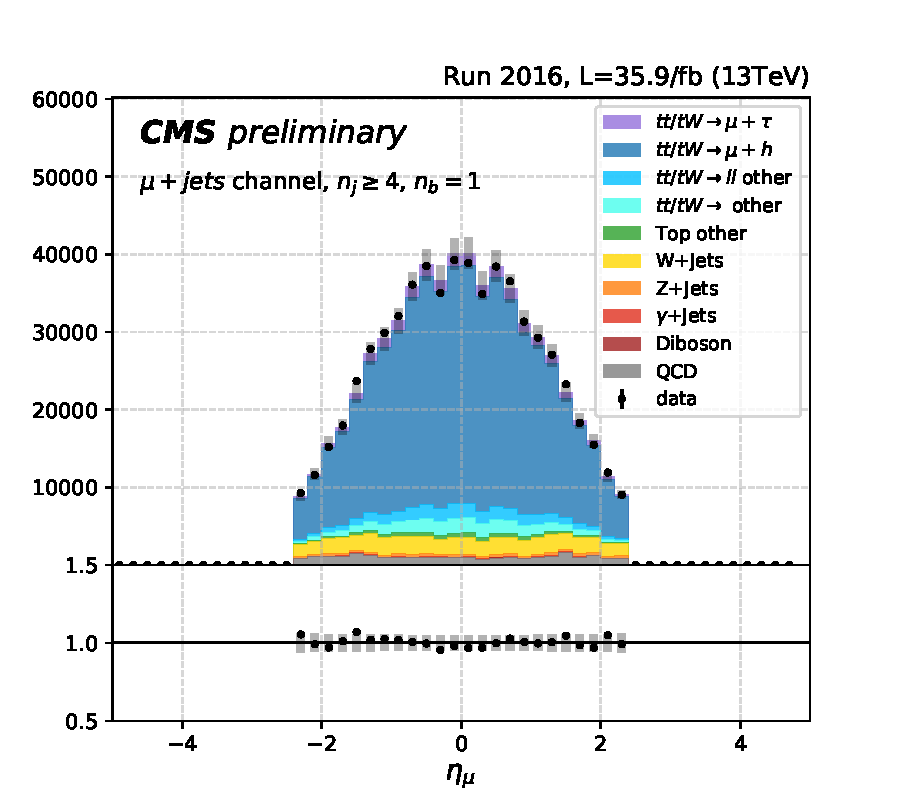
\includegraphics[width=0.49\textwidth]{chapters/Analysis/sectionPlots/figures/kinematics_pickles/mu4j/1b/mu4j_1b_lepton1_eta.pdf}
    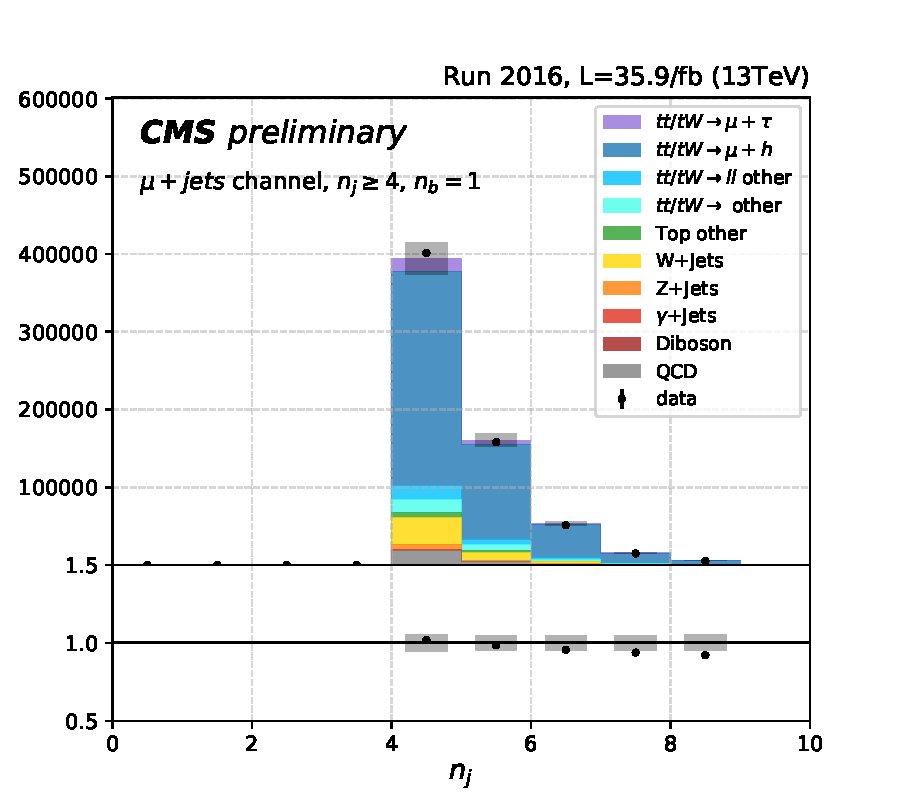
\includegraphics[width=0.49\textwidth]{chapters/Analysis/sectionPlots/figures/kinematics_pickles/mu4j/1b/mu4j_1b_nJets.pdf}
    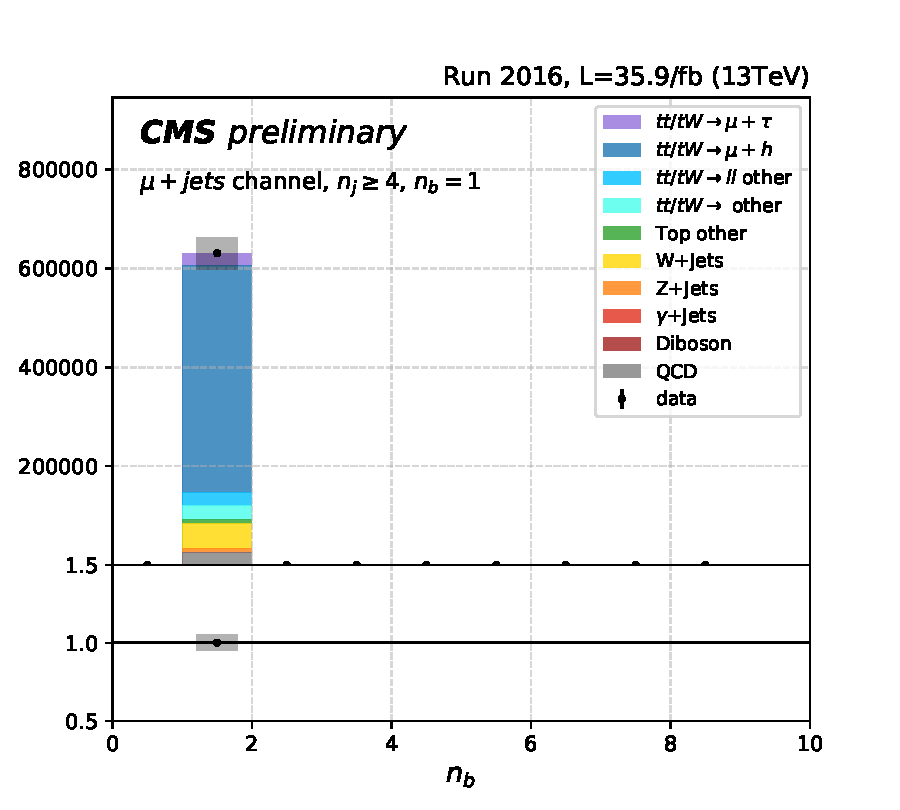
\includegraphics[width=0.49\textwidth]{chapters/Analysis/sectionPlots/figures/kinematics_pickles/mu4j/1b/mu4j_1b_nBJets.pdf}
    
    \caption{$\mu$jet channel with $n_j\geq4, n_b=1$.}
\end{figure}

\begin{figure}[ht]
    \centering
    $\mu j - 2b$ \\
    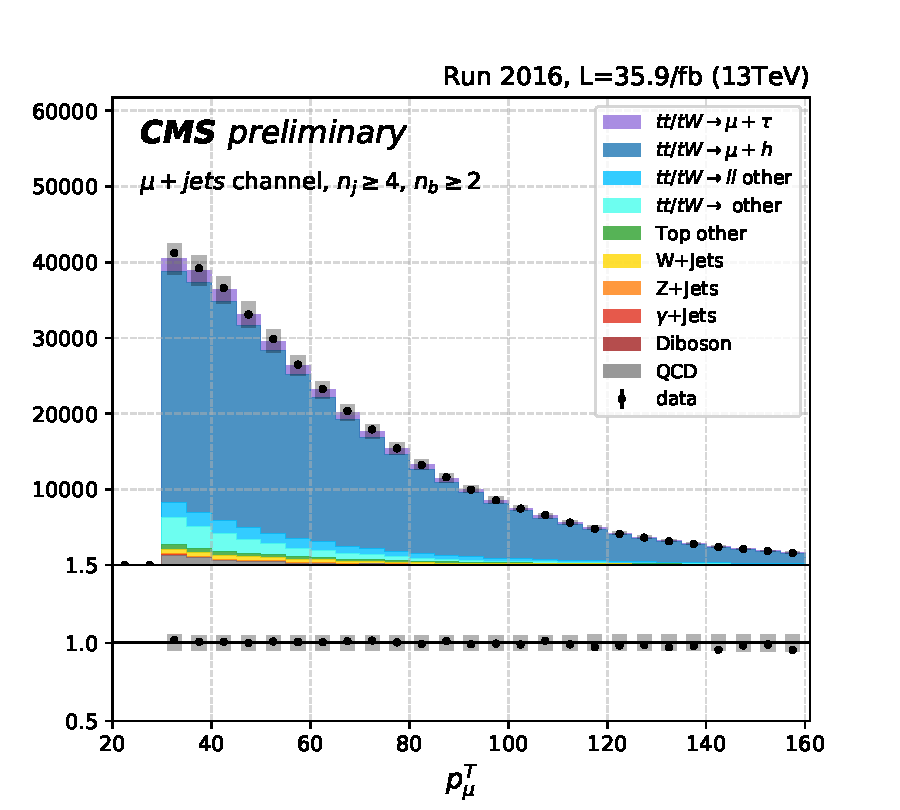
\includegraphics[width=0.49\textwidth]{chapters/Analysis/sectionPlots/figures/kinematics_pickles/mu4j/2b/mu4j_2b_lepton1_pt.pdf}
    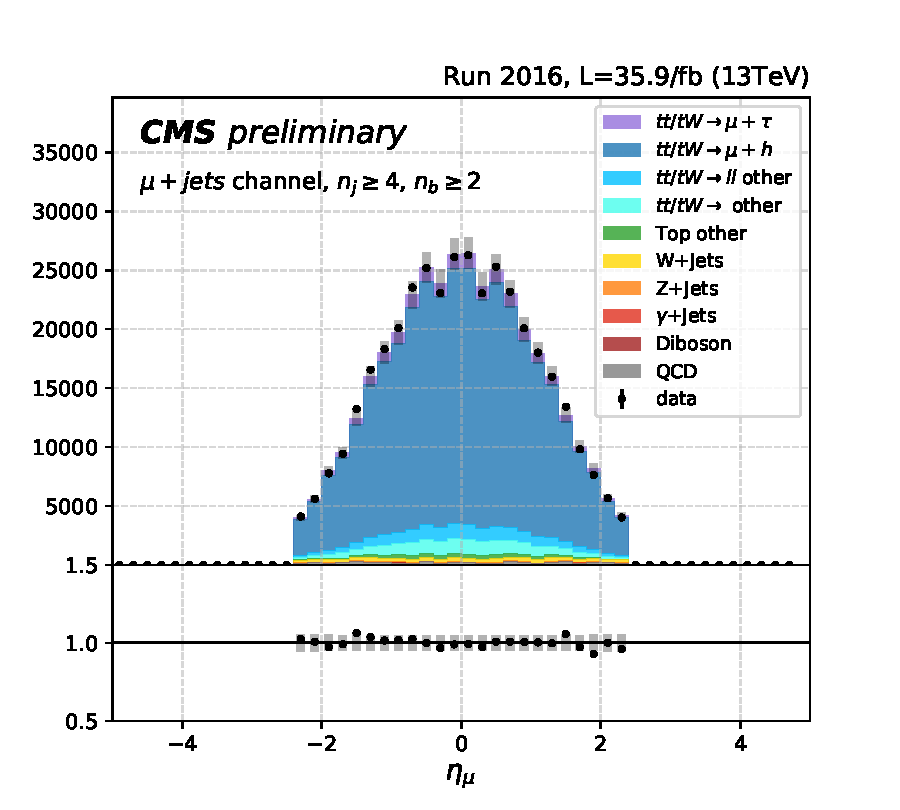
\includegraphics[width=0.49\textwidth]{chapters/Analysis/sectionPlots/figures/kinematics_pickles/mu4j/2b/mu4j_2b_lepton1_eta.pdf}
    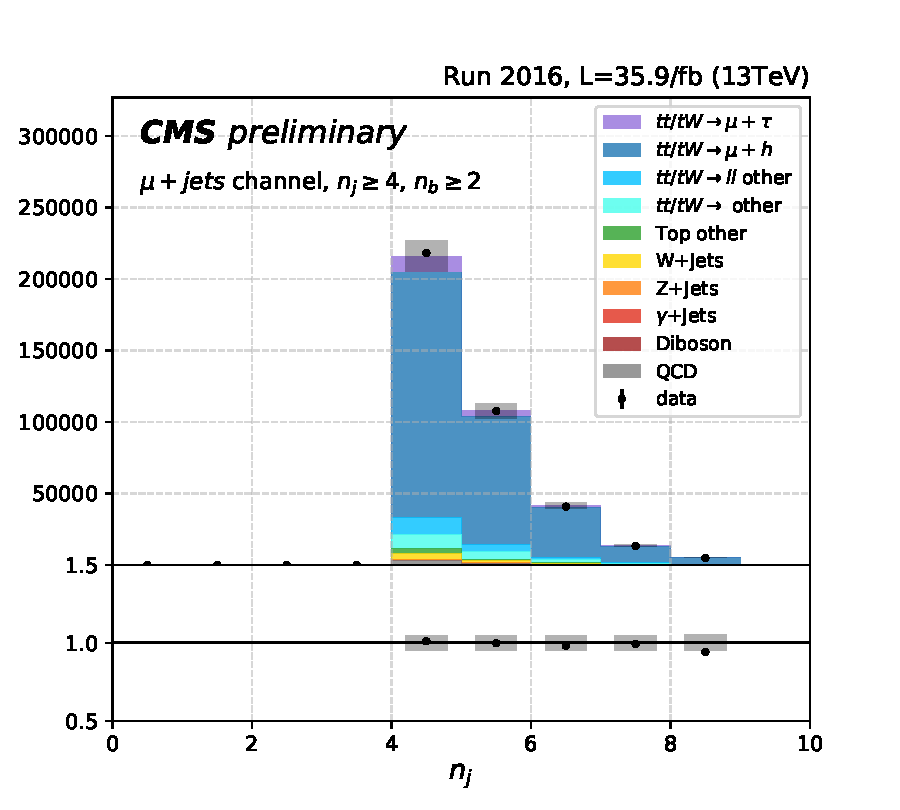
\includegraphics[width=0.49\textwidth]{chapters/Analysis/sectionPlots/figures/kinematics_pickles/mu4j/2b/mu4j_2b_nJets.pdf}
    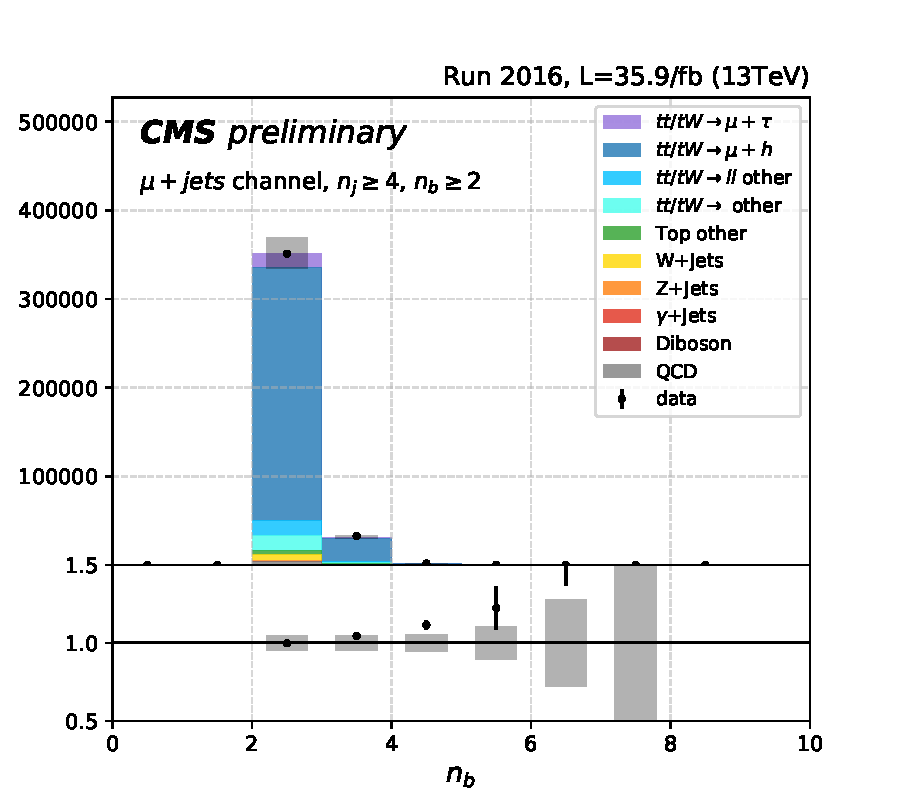
\includegraphics[width=0.49\textwidth]{chapters/Analysis/sectionPlots/figures/kinematics_pickles/mu4j/2b/mu4j_2b_nBJets.pdf}
    
    \caption{$\mu$jet channel with $n_j\geq4, n_b\geq2$.}
\end{figure}













%  ee channel
\begin{figure}[ht]
    \centering
    $ee - 1b$ \\
    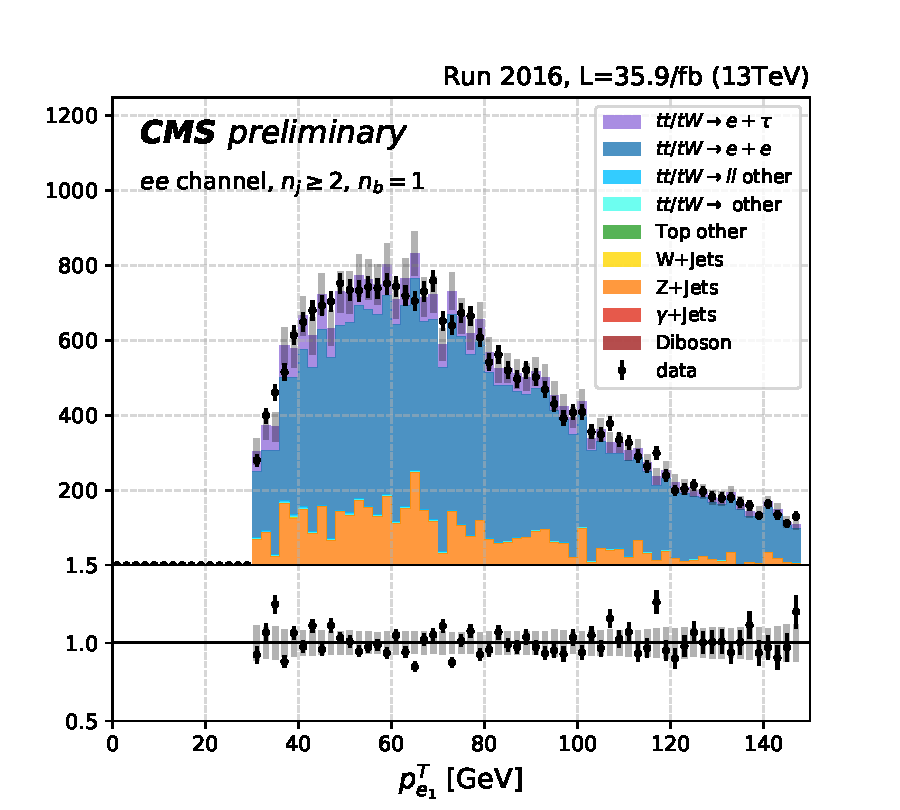
\includegraphics[width=0.49\textwidth]{chapters/Analysis/sectionPlots/figures/kinematics_pickles/ee/1b/ee_1b_lepton1_pt.pdf}
    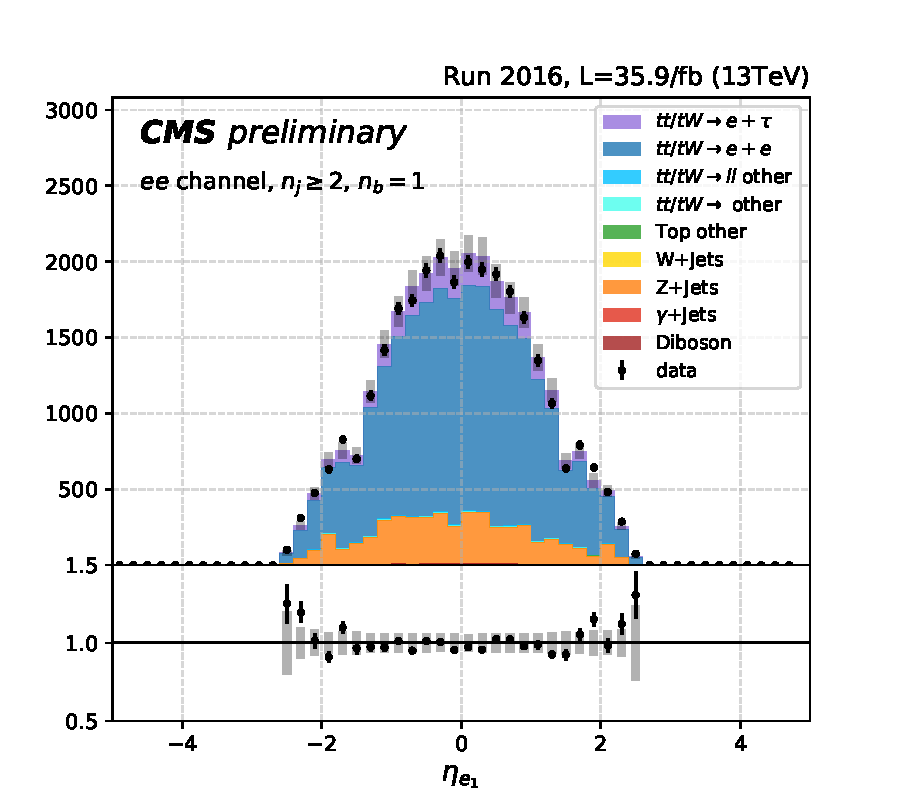
\includegraphics[width=0.49\textwidth]{chapters/Analysis/sectionPlots/figures/kinematics_pickles/ee/1b/ee_1b_lepton1_eta.pdf}
    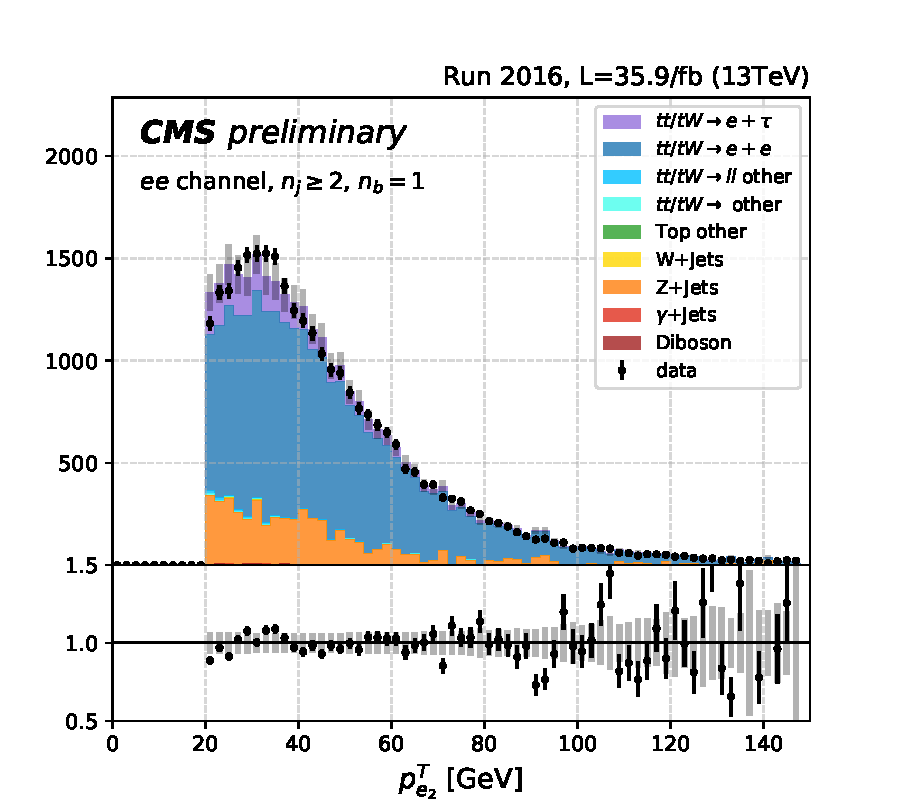
\includegraphics[width=0.49\textwidth]{chapters/Analysis/sectionPlots/figures/kinematics_pickles/ee/1b/ee_1b_lepton2_pt.pdf}
    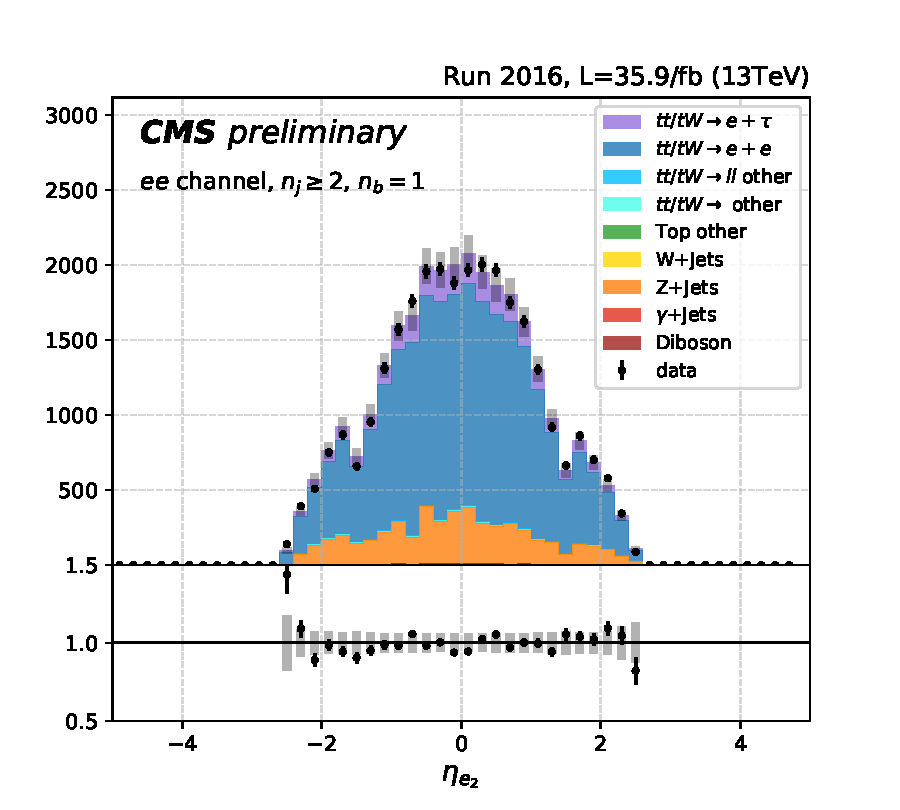
\includegraphics[width=0.49\textwidth]{chapters/Analysis/sectionPlots/figures/kinematics_pickles/ee/1b/ee_1b_lepton2_eta.pdf}
    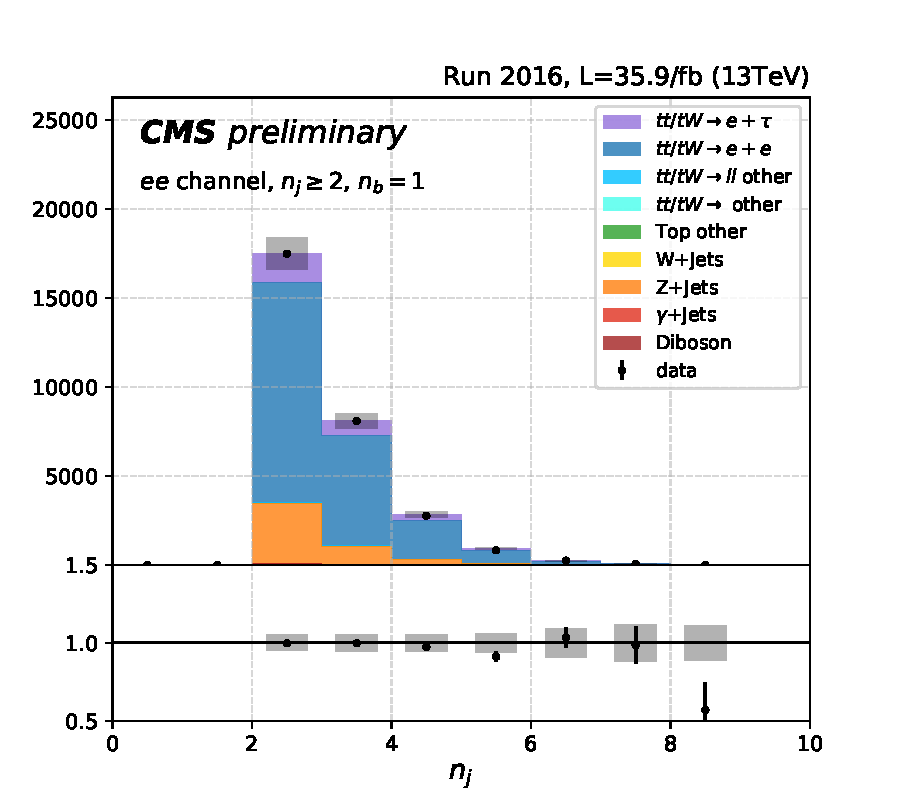
\includegraphics[width=0.49\textwidth]{chapters/Analysis/sectionPlots/figures/kinematics_pickles/ee/1b/ee_1b_nJets.pdf}
    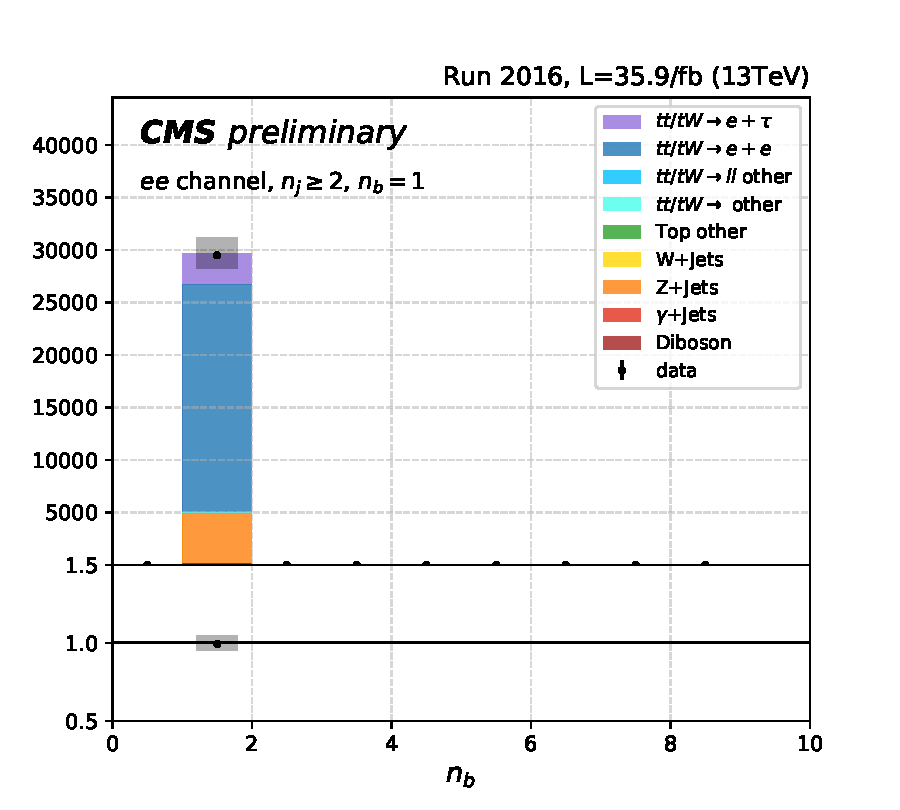
\includegraphics[width=0.49\textwidth]{chapters/Analysis/sectionPlots/figures/kinematics_pickles/ee/1b/ee_1b_nBJets.pdf}
    
    \caption{$ee$ channel with $n_j\geq4, n_b=1$.}
\end{figure}

\begin{figure}[ht]
    \centering
    $ee - 2b$ \\
    \includegraphics[width=0.49\textwidth]{chapters/Analysis/sectionPlots/figures/kinematics_pickles/ee/2b/ee_2b_lepton1_pt.pdf}
    \includegraphics[width=0.49\textwidth]{chapters/Analysis/sectionPlots/figures/kinematics_pickles/ee/2b/ee_2b_lepton1_eta.pdf}
    \includegraphics[width=0.49\textwidth]{chapters/Analysis/sectionPlots/figures/kinematics_pickles/ee/2b/ee_2b_lepton2_pt.pdf}
    \includegraphics[width=0.49\textwidth]{chapters/Analysis/sectionPlots/figures/kinematics_pickles/ee/2b/ee_2b_lepton2_eta.pdf}
    \includegraphics[width=0.49\textwidth]{chapters/Analysis/sectionPlots/figures/kinematics_pickles/ee/2b/ee_2b_nJets.pdf}
    \includegraphics[width=0.49\textwidth]{chapters/Analysis/sectionPlots/figures/kinematics_pickles/ee/2b/ee_2b_nBJets.pdf}
    
    \caption{$ee$ channel with $n_j\geq2, n_b\geq2$.}
\end{figure}

%  emu channel
\begin{figure}[ht]
    \centering
    $e \mu - 1b$ \\
    \includegraphics[width=0.49\textwidth]{chapters/Analysis/sectionPlots/figures/kinematics_pickles/emu2/1b/emu2_1b_lepton1_pt.pdf}
    \includegraphics[width=0.49\textwidth]{chapters/Analysis/sectionPlots/figures/kinematics_pickles/emu2/1b/emu2_1b_lepton1_eta.pdf}
    \includegraphics[width=0.49\textwidth]{chapters/Analysis/sectionPlots/figures/kinematics_pickles/emu2/1b/emu2_1b_lepton2_pt.pdf}
    \includegraphics[width=0.49\textwidth]{chapters/Analysis/sectionPlots/figures/kinematics_pickles/emu2/1b/emu2_1b_lepton2_eta.pdf}
    \includegraphics[width=0.49\textwidth]{chapters/Analysis/sectionPlots/figures/kinematics_pickles/emu2/1b/emu2_1b_nJets.pdf}
    \includegraphics[width=0.49\textwidth]{chapters/Analysis/sectionPlots/figures/kinematics_pickles/emu2/1b/emu2_1b_nBJets.pdf}
    
    \caption{$e\mu$ channel with $n_j\geq4, n_b=1$.}
\end{figure}

\begin{figure}[ht]
    \centering
    $e\mu - 2b$ \\
    \includegraphics[width=0.49\textwidth]{chapters/Analysis/sectionPlots/figures/kinematics_pickles/emu2/2b/emu2_2b_lepton1_pt.pdf}
    \includegraphics[width=0.49\textwidth]{chapters/Analysis/sectionPlots/figures/kinematics_pickles/emu2/2b/emu2_2b_lepton1_eta.pdf}
    \includegraphics[width=0.49\textwidth]{chapters/Analysis/sectionPlots/figures/kinematics_pickles/emu2/2b/emu2_2b_lepton2_pt.pdf}
    \includegraphics[width=0.49\textwidth]{chapters/Analysis/sectionPlots/figures/kinematics_pickles/emu2/2b/emu2_2b_lepton2_eta.pdf}
    \includegraphics[width=0.49\textwidth]{chapters/Analysis/sectionPlots/figures/kinematics_pickles/emu2/2b/emu2_2b_nJets.pdf}
    \includegraphics[width=0.49\textwidth]{chapters/Analysis/sectionPlots/figures/kinematics_pickles/emu2/2b/emu2_2b_nBJets.pdf}
    
    \caption{$e\mu$ channel with $n_j\geq2, n_b\geq2$.}
\end{figure}


%  etau channel
\begin{figure}[ht]
    \centering
    $e\tau - 1b$ \\
    \includegraphics[width=0.49\textwidth]{chapters/Analysis/sectionPlots/figures/kinematics_pickles/etau/1b/etau_1b_lepton1_pt.pdf}
    \includegraphics[width=0.49\textwidth]{chapters/Analysis/sectionPlots/figures/kinematics_pickles/etau/1b/etau_1b_lepton1_eta.pdf}
    \includegraphics[width=0.49\textwidth]{chapters/Analysis/sectionPlots/figures/kinematics_pickles/etau/1b/etau_1b_lepton2_pt.pdf}
    \includegraphics[width=0.49\textwidth]{chapters/Analysis/sectionPlots/figures/kinematics_pickles/etau/1b/etau_1b_lepton2_eta.pdf}
    \includegraphics[width=0.49\textwidth]{chapters/Analysis/sectionPlots/figures/kinematics_pickles/etau/1b/etau_1b_nJets.pdf}
    \includegraphics[width=0.49\textwidth]{chapters/Analysis/sectionPlots/figures/kinematics_pickles/etau/1b/etau_1b_nBJets.pdf}
    
    \caption{$e\tau$ channel with $n_j\geq4, n_b=1$.}
\end{figure}

\begin{figure}[ht]
    \centering
    $e\tau - 2b$ \\
    \includegraphics[width=0.49\textwidth]{chapters/Analysis/sectionPlots/figures/kinematics_pickles/etau/2b/etau_2b_lepton1_pt.pdf}
    \includegraphics[width=0.49\textwidth]{chapters/Analysis/sectionPlots/figures/kinematics_pickles/etau/2b/etau_2b_lepton1_eta.pdf}
    \includegraphics[width=0.49\textwidth]{chapters/Analysis/sectionPlots/figures/kinematics_pickles/etau/2b/etau_2b_lepton2_pt.pdf}
    \includegraphics[width=0.49\textwidth]{chapters/Analysis/sectionPlots/figures/kinematics_pickles/etau/2b/etau_2b_lepton2_eta.pdf}
    \includegraphics[width=0.49\textwidth]{chapters/Analysis/sectionPlots/figures/kinematics_pickles/etau/2b/etau_2b_nJets.pdf}
    \includegraphics[width=0.49\textwidth]{chapters/Analysis/sectionPlots/figures/kinematics_pickles/etau/2b/etau_2b_nBJets.pdf}
    
    \caption{$e\tau$ channel with $n_j\geq2, n_b\geq2$.}
\end{figure}


% ej channel
\begin{figure}[ht]
    \centering
    $e j- 1b$ \\
    \includegraphics[width=0.49\textwidth]{chapters/Analysis/sectionPlots/figures/kinematics_pickles/e4j/1b/e4j_1b_lepton1_pt.pdf}
    \includegraphics[width=0.49\textwidth]{chapters/Analysis/sectionPlots/figures/kinematics_pickles/e4j/1b/e4j_1b_lepton1_eta.pdf}
    \includegraphics[width=0.49\textwidth]{chapters/Analysis/sectionPlots/figures/kinematics_pickles/e4j/1b/e4j_1b_nJets.pdf}
    \includegraphics[width=0.49\textwidth]{chapters/Analysis/sectionPlots/figures/kinematics_pickles/e4j/1b/e4j_1b_nBJets.pdf}
    
    \caption{$e$jet channel with $n_j\geq4, n_b=1$.}
\end{figure}

\begin{figure}[ht]
    \centering
    $e j - 2b$ \\
    \includegraphics[width=0.49\textwidth]{chapters/Analysis/sectionPlots/figures/kinematics_pickles/e4j/2b/e4j_2b_lepton1_pt.pdf}
    \includegraphics[width=0.49\textwidth]{chapters/Analysis/sectionPlots/figures/kinematics_pickles/e4j/2b/e4j_2b_lepton1_eta.pdf}
    \includegraphics[width=0.49\textwidth]{chapters/Analysis/sectionPlots/figures/kinematics_pickles/e4j/2b/e4j_2b_nJets.pdf}
    \includegraphics[width=0.49\textwidth]{chapters/Analysis/sectionPlots/figures/kinematics_pickles/e4j/2b/e4j_2b_nBJets.pdf}
    
    \caption{$e$jet channel with $n_j\geq2, n_b\geq2$.}
\end{figure}
